\newpage
\chapter{NÖTRİNO SALINIM KİNEMATİĞİ}\label{ch:nuHareketKinematik}
\paragraph{}
Nötrinolar kütleli, ışık hızına yakın hızlarda giden ve Fermi-Dirac istatistiğine sahip olan parçacıklardır. Nötrinoların çeşni evrimi Schrödinger tipi denklem ile verilir \cite{Raffelt:1996wa}. 
\begin{equation}\label{eqn:NuKim_EoM_Psi}
	i\dv{r} \ket{\Psi(r)}= H^{\text{f}}(r) \ket{\Psi(r)} \text{ .}
\end{equation}
Burada $ \ket{\Psi(r)} $ nötrino durum (state) keti veya vektörü $ H^{\text{f}} $ çeşni tabanında yazılmış Hamiltonyen'dir. Hareket denklemi Schrödinger tipi diferansiyel denklem ile yazılabileceği gibi integral denklemleri şeklinde de yazılabilir \cite{Kneller:2005hf}. Bu tezde, dört ($ 2 $ nötrino, $ 2 $ antinötrino) çeşni dikkate alınacaktır. \eqref{eqn:NuKim_EoM_Psi} numaralı hareket denklemi nötrino çeşni ketlerine göre aşağıdaki gibi olur.
\begin{equation}\label{eqn:NuKim_EoM_4Mat}
	i\dv{r} \mqty(\ket{\nu_{e}(r)} \\ \ket{\nu_{\mu}(r)}\\ \ket{\nu_{\overline{e}}(r)}\\ \ket{\nu_{\overline{\mu}}(r)}) = H^{\text{f}}(r) \mqty(\ket{\nu_{e}(r)} \\ \ket{\nu_{x}(r)}\\ \ket{\nu_{\overline{e}}(r)}\\ \ket{\nu_{\overline{x}}(r)}) \text{ .}
\end{equation}
Bu denklemdeki durum vektörü, çeşni bazında yazılmıştır. $ x $ olarak etiketlenen nötrinolar müon ve tau çeşnilerinin bir kombinasyonu olarak düşünülür. Üniter dönüşümler kullanılarak \eqref{eqn:NuKim_EoM_4Mat} numaralı denklem başka bazlara çevrilebilir.

Astrofiziksel ortamdaki parçacıkların davranışlarını tek tek incelemek imkansızdır. Bunun yerine onların toplu davranışlarını incelemek daha uygun olur. Bunun için nötrino parçacığının evrimini veren Schrödinger denklemini çözüp durum vektörünü elde etmek yerine yoğunluk operatörü formalizmine geçilir. Yoğunluk operatörü formalizmi nötrinoların istatistiksel dağılımının evrimine bakabilmemize olanak verir. \eqref{eqn:NuKim_EoM_Psi} numaralı denklemin $ \ket{\Psi_{1}(r)} $ için yazıldığını varsayalım. Ardından \eqref{eqn:NuKim_EoM_Psi} numaralı denklemi sağdan $ a_{1}\bra{\Psi_{1}(r)} $ ile çarpalım. Aynı işlemi $ \ket{\Psi_{2}(r)} $ için de yapıp alt alta $ i $ kere toplarsak aşağıdaki ifadeyi elde ederiz.
\begin{equation}
	i\dv{r} \qty(\sum_{i} a_{i} \dyad{\Psi_{i}(r)}{\Psi_{i}(r)})  = \comm{H^{\text{f}}(E,r)}{\sum_{i} a_{i} \dyad{\Psi_{i}(r)}{\Psi_{i}(r)} } \text{ .}
\end{equation}

Artık yoğunluk operatörünü tanımlayabiliriz.
\begin{equation} \label{eqn:NuKim_YogOperatorTanım}
	\hat{\rho} (r) = \sum_{i} a_{i} \dyad{\Psi_{i}(r)}{\Psi_{i}(r)}  \text{ .}
\end{equation}
Burada $ a_{i} $ bir sayıdır ve sistemde ne oranda $ \ket{\Psi_{i}(r)} $ durumu olduğunu betimler. Yani iki durumlu sistem için $ a_{1}=N_{1}/(N_{1}+N_{2}) $ şeklinde yazılır. Yoğunluk operatörünü hareket denklemine koyduğumuzda \emph{Liouville - von Neumann} denklemini elde ederiz. 
\begin{equation}\label{eqn:NuKim_LiouvilleVonNeumann}
	i \dv{r} \hat{\rho} = \comm{\hat{H}}{\hat{\rho}} \text{ .}
\end{equation}
Bu denklem Heisenberg Denklemine benzemektedir ancak Liouville - von Neumann denkleminde operatörler değil durumlar evrilir. Buna ek olarak eksi işaret farkı da vardır. Liouville - von Neumann denkleminin sağ tarafına çarpışma (collision) katkıları da yazılabilir \cite{Volpe:2015rla}. Bu çalışmada çarpışma terimleri ihmal edilecektir. Denklemin sol tarafı ise konuma göre tam türev içerir. Yani $ \dv{r} = \pdv{r} + \vec{v} \cdot \vec{\nabla} $ şeklinde yazılır. Bu çalışmada yoğunluk operatörü açıdan bağımsız bir şekilde evrilecektir. Bundan dolayı hız, $ \vec{v} $, ile bağlı olan tüm terimler düşecektir. Geometri hakkında ayrıntılı bilgi için \ref{subsec:geometri} numaralı bölüme bakabilirsiniz.

Yoğunluk operatöründen yoğunluk matrisine geçmek için bir baz seçilmesi gerekmektedir. Örneğin, çeşni bazını, $ \ket{\nu_{\alpha}} $, ele alalım. Bunun için \eqref{eqn:NuKim_YogOperatorTanım} numaralı denkleme iki adet tam küme (complete set) koymamız gerekir.
\begin{equation}
	\hat{\rho}(r) = \sum_{\alpha,\beta} \rho_{\alpha\beta}(r) \dyad{\nu_{\alpha}}{\nu_{\beta}} \text{ .}
\end{equation}
Burada $ \rho_{\alpha\beta}(r) $ yoğunluk matrisidir ve aşağıdaki gibi tanımlanır.
\begin{equation}
	\rho_{\alpha\beta}(r) = \sum_{i} a_{i}\braket{\nu_{\alpha}}{\Psi_{i}(r)}\braket{\Psi_{i}(r)}{\nu_{\beta}}
\end{equation}
$ a_{i} $, topluluğun (ensemble) içerisindeki nötrino çeşnilerinin (diğer bazlarda da tanımlanabilir) ağırlığını vermektedir. Yoğunluk matrisi tanımlanan baza göre değişiklik gösterir. Evrim ise yoğunluk operatörü ile ilişkili olduğu için seçilen bazdan bağımsızdır. Yani fiziksel evrim, seçilen bazdan bağımsızdır.

Yoğunluk matrisine örnek olarak iki durumlu nötrinoları ele alabiliriz. Örneğin, $ \ket{\nu_{e}} = \mqty(1\\0) $ ve $ \ket{\nu_{x}} = \mqty(0\\1) $ olsun. Bu durumda yoğunluk operatörü şöyle yazılır.
\begin{equation}
	\hat{\rho}(r) = \mqty(\rho_{ee}(r) & \rho_{ex}(r) \\\rho_{xe}(r) & \rho_{xx}(r)) \text{ .}
\end{equation}
Yoğunluk matrisi saf (pure) ve karışık (mixed) olmak üzere iki çeşit olabilir. Saf durumlar sadece aynı cins durumların bir araya gelmesiyle oluşur. Karışık durumlarda ise farklı kombinasyonlara sahip durumlar da olabilir. Bu çalışmada, başlangıçtaki yoğunluk matrisi her zaman saf durumda olacaktır.

Yoğunluk matrisinin temel özellikleri evrimin kavramsal olarak anlaşılmasını kolaylaştırır. Yoğunluk matrisinin izi birdir. Bu da topluluğun içerisindeki toplam maddenin korunduğu anlamına gelir. Yani toplulukta $ a_{1} $ oranında $ \ket{\Psi_{1}} $ parçacığı, $ a_{2} $ oranında $ \ket{\Psi_{2}} $ olsun. Başlangıçta $ a_{1}+a_{2} =1 $ olarak verilir. Bu toplamın evrimin her anında aynı olması beklenir. Yoğunluk matrisinin her bir köşegen elemanı ise yaşama olasılığı (survival probability) ile orantılıdır. Örneğin, saf bir durumda, yoğunluk matrisinin $ \rho_{ee}(r) $ elemanı, hayata elektron nötrinosu olarak başlayıp $ r $ uzaklığında hala elektron nötrinosu olma olasılığının $ a_{e} $ ile çarpımını verir. Benzer şekilde köşegen olmayan elemanlar da geçiş olasılığı ile orantılıdır. Yoğunluk matrisinin izinin bir olmasının yanında üst köşegen elemanları ile alt köşegen elemanları birbirinin sanal eşleniğidir (complex conjugate.) Yoğunluk matrisinin diğer özellikleri ve uygulamaları \cite{2012dmta.book.....B} numaralı kaynakta ayrıntılı olarak verilmiştir.

Nötrino durumu, $ \ket{\Psi(r)} $, başlangıçta Hamiltonyen'in özvektörleri cinsinden yazalım. Sistemin başlangıçtaki özvektörleri de $ \ket{E_{i}(R)} $ olarak gösterilsin. Burada durum, tek bir özvektöre eşit olabildiği gibi birden çok öz durumun doğrusal kombinasyonu da olabilir. Eğer nötrino durumu, evrim boyunca fazladan bir faz ile beraber Hamiltonyen'in özbazında kalıyorsa, evrime \emph{adyabatiktir} denir. Adyabatik evrimde, herhangi bir $ r $ uzaklığında nötrino durumu aşağıdaki gibi yazılır.
\begin{equation}\label{eqn:Psi_rAdiabaticPhase}
    \ket{\Psi(r)} = \sum_{i} e^{-i \int^{r}_{R} E_{i}(r') \dd{r'}} \ket{E_{i}(r)} \text{ .}
\end{equation}
Burada $ E_{i}(r') $ Hamiltonyen'in özdeğeridir. Yoğunluk operatörünün özbazdaki hali aşağıdaki gibi yazılır.
\begin{equation}\label{eqn:rhoHat_rAdiabaticPhase}
    \hat{\rho}(r) = \sum_{i,j} \rho_{ij}(R) e^{-i \int^{r}_{R} \qty(E_{i}(r')-E_{j}(r')) \dd{r'}} \dyad{E_{i}(r)}{E_{j}(r)} \text{ .}
\end{equation}
Eğer yoğunluk matrisi, başlangıçta köşegen, bir diğer değişle $ \eval{\rho_{ab}(R)}_{a\ne b}=0  $ ise eksponansiyel faz yok olacaktır. Adyabatik ve diyabatik (adyabatik olmayan) evrimler ilerleyen bölümlerde daha ayrıntılı incelenecektir.

Tezin bu kısmından itibaren tüm denklemler iki çeşni gözetilerek ($ e,x,\bar{e},\bar{x} $) yazılacaktır. Efektif olarak iki çeşni almak teorik hesapların daha kolay yapılması için önemlidir. Buna ek olarak nötrinoların ve antinötrinoların ait olduğu denklemlerin ayrılamadığı durumlar için nötrino durum vektörü $ 4 $ boyutlu olacaktır. Bu da teorik olarak yapılan hesapları daha da karmaşık hale getireceği için çeşitli varsayımlarda bulunulacaktır.

Nötrinoların Majorana doğasına sahip olduğu varsayılacaktır. Bu varsayım altında, Dirac nötrinoları varsayıldığında dört olan serbestlik derecesi ikiye düşecektir. Majorana parçacıkları için parçacık - antiparçacık ayrımı yoktur. Bunun yerine parçacıklara, sağ elli veya sol elli parçacıklar demek doğrudur. Tezin bu kısmından itibaren sol elli nötrinolar demek yerine nötrinolar, sağ elli nötrinolar demek yerine antinötrinolar denecektir. Majorana ve Dirac nötrinoları için daha ayrıntılı bilgi \cite{Bilenky:2020vjk} numaralı kaynakta anlatılmıştır.

\section{BOŞLUK SALINIMLARI}\label{sec:boslukSalinimlari}
\paragraph{}
Standart Model'de nötrinolar kütlesiz parçacıklardır. Nötrinoların Standart Model'de sadece sol elli olarak var olmasından kaynaklıdır. SM'de nötrinolar ışık hızında giden "kütlesiz" parçacıklar olduğu için kiralite ve helisite aynı anlama gelir. Nötrinolara kütle verme mekanizması pariteyi açıkça ihlal eder ve Higgs Mekanizmasıyla nötrinolara kütle vermeyi olanaksız kılar. Bu nedenle nötrinolara "standart" bir biçimde kütle vermek imkansızdır. Bir diğer taraftan, deneylerle defalarca kanıtlanan nötrino salınımlarının teorisi yazıldığında, salınım frekansının kütle kare farkları ile doğru orantılı olduğu görülür. Bu da en az bir nötrino özdurumunun kütleli olması gerektiği anlamına gelir. Bu bakımdan nötrinoların çeşni salınımı standart model ötesi teoriler arasında çok önemli bir yer teşkil eder. 

Bu bölümde nötrino salınımlarının teorisi ele alınacaktır. Salınımların alan teorisindeki tasviri \cite{2010arXiv1011.4300D} değil, kuantum mekaniği tasviri \cite{raffelt1996stars} kullanılacaktır.

Nötrinolar ve antinötrinolar boşlukta ilerlerken (propagation) özbazı kütle tabanıdır. Yani boşluktaki nötrinolar kütle tabanında iyi tanımlıdır (well-defined). Tabandan bağımsız olarak Hamiltonyen operatörünü tanımlayabiliriz.
\begin{align} \label{eqn:NuKim_BoslukSal_Hnu_op}
	\nonumber \hat{H}_{\nu} & = \hat{H}_{\text{n\"{o}trino}} + \hat{H}_{\text{antin\"{o}trino}}\\
						    & = \sum^{4}_{i=1}\frac{m_{i}^{2}}{2E} \dyad{\nu_{i}}{\nu_{i}}\text{ .}
\end{align}
Burada $ 1,2 $ nötrinoları ve $ 3,4 $ antinötrinoları temsil etmektedir. Bu çalışmada,\emph{CP simetrisinin} kırılmadığı durumlar ele alınacaktır. Yani CP fazını sıfır alacağız. Bundan dolayı nötrinolar ve antinötrinolar aynı şekilde çeşnilerini dönüştürecek ve aynı kütle özdurumlarına sahip olacaklardır. Matematiksel olarak da özdeğerleri aynı olmalıdır $ m^{2}_{1,2} = m^{2}_{3,4} $. Çeşni tabanı ile kütle tabanı arasındaki geçiş dönme matrisi cinsinden yazılabilir. 
\begin{align}\label{eqn:NuKim_BoslukSal_ketEketX}
	\ket{\nu_{e}} & =  \cos \theta \ket{\nu_{1}} + \sin \theta \ket{\nu_{2}} \text{ ,} \\
	\ket{\nu_{x}} & = -\sin \theta \ket{\nu_{1}} + \cos \theta \ket{\nu_{2}} \text{ .}
\end{align}
Burada $ \theta $ boşluk salınım açısıdır. Hem kütle bazında hem de çeşni bazında özdurumlar birbirine diktir, $\abs{\braket{\nu_{\alpha}}{\nu_{\beta}}}=\delta_{\alpha\beta} $, $ \abs{\braket{\nu_{i}}{\nu_{j}}}=\delta_{ij} $. Yukarıdaki dönüşümlerin aynısı antinötrinolar için de yazılır. Bu dönüşümler özel bir baz seçmeden matris formunda da yazılabilir. 
\begin{equation}
	\mqty(\ket{\nu_{e}} \\ \ket{\nu_{x}} ) = U \mqty(\ket{\nu_{1}} \\ \ket{\nu_{2}} ) \text{ .}
\end{equation}
$ U $, karışımı veren dönme matrisi olarak yazılabilir. Nötrinolar ve antinötrinolar için aynı $ U $ matrisi geçerlidir. 

Nötrinolar sadece çeşni tabanında etkileşime girdiklerinden dolayı etkileşim tabanı çeşni tabanıdır. Bu durum nötrinoların kütlesi ve çeşnisini tanımlayan leptonlar arasında bir kafa karışıklığına yol açar. Herhangi bir etkileşime girmeyen nötrinolar boşlukta ilerlerken çeşni değiştiriyorsa kütle kazanmış gibi gözükmektedir. Bu sav örneğin, müon nötrinosunun elektron nötrinosundan ağır olması şartıyla ortaya konabilir. Bu kafa karışıklığı elektron nötrinosunun kütle tanımı ile çözülür. \eqref{eqn:NuKim_BoslukSal_ketEketX} denklemlerine göre \emph{elektron} çeşnisine sahip nötrinonun öz durumu iki farklı kütle özdurumunun bir süperpozisyonu (superposition) şeklinde yazılmaktadır. Bundan dolayı elektron nötrinosunun kütlesi iyi tanımlı bir kavram değildir. Bazı yazarlar kuark salınımlarına gönderme yaparak nötrino salınımı yerine lepton salınımı ifadesini kullanmaktadır \cite{Kayser:2001ki}. Ayrıca nötrino salınımları ile ilgili "paradokslar" için \cite{Akhmedov:2009rb} numaralı kaynağa bakınız.

Eğer nötrinoları ve antinötrinoları aynı denklem içerisinde yazmak istersek, $ U $ matrisinin boyutunu arttırmamız gerekmektedir.
\begin{equation}
	\mqty(\ket{\nu_{e}} \\ \ket{\nu_{x}} \\ \ket{\nu_{\bar{e}}} \\ \ket{\nu_{\bar{x}}} ) = U \mqty(\ket{\nu_{1}} \\ \ket{\nu_{2}} \\\ket{\nu_{\bar{1}}} \\ \ket{\nu_{\bar{2}}}) \text{ .}
\end{equation}

Yeni $ U $ matrisi aşağıdaki gibi tanımlanır.
\begin{equation}\label{eqn:BoslukSal_DonusumMat}
	U= \mqty( \cos \theta & \sin \theta & 0 & 0 \\ -\sin \theta & \cos \theta & 0 & 0 \\ 0 & 0 & \cos \theta & \sin \theta\\ 0 & 0 & - \sin \theta & \cos \theta)
\end{equation}

$ U $ dönüşüm matrisi nötrino enerjisine ve uzaklığına bağlı değildir. Yani statik bir dönme matrisidir. $ U $ matrisi dönme matrisleri, $ \mathcal{R}_{\theta} $, kullanmadan da tanımlanabilir ancak literatürde karışım açısı tanımlamak en yaygın yaklaşımdır \cite{ParticleDataGroup:2018ovx}. Dönüşüm matrisleri üniter olmak zorundadır, $ U U^{\dagger} = U^{\dagger} U = \mathbb{1}$. $ U $ matrisini gerçel (reel) almak CP simetri kırılım fazını sıfır almak ile eşdeğerdir. CP kırılım fazı tezin bu anından itibaren sıfır alınacaktır. Sıfır $ \delta_{CP} $ fazı almak, üniterlik koşulunu ortogonallik koşuluna indirger. $ U U^{T} = \mathbb{1} $. $ U $ matrisinin $ \alpha,i $ bileşeni braket notasyonu ile de tanımlanabilir, $ U_{\alpha i} =\braket{\nu_{\alpha}}{\nu_{i}} $. Bu dönüşüm daha kapalı yani kompakt bir şekilde yazmak mümkündür \cite{ParticleDataGroup:2018ovx}.
\begin{equation} \label{eqn:BoslukSal_GecisBraKet}
	\ket{\nu_{\alpha}} = \sum_{i=1,2,3,4} U_{\alpha i} \ket{\nu_{i}}\text{,} \quad \ket{\nu_{i}} = \sum_{i=e,x,\overline{e},\overline{x}} U_{\alpha i} \ket{\nu_{\alpha}} \text{ .}
\end{equation}

$ U $ matrisinde satırlar çeşniler üzerinden sıralanır, sütunlar ise kütle üzerinden sıralanır. Aksi belirtilmedikçe çeşni bazı ile alakalı ifadelere $ \alpha,\beta $ etiketleri verilecektir.

\eqref{eqn:NuKim_BoslukSal_Hnu_op} numaralı Hamiltonyen operatörü kütle bazında yazılmıştır. \emph{Aynı} Hamiltonyen \eqref{eqn:BoslukSal_GecisBraKet} numaralı denklem kullanılarak çeşni bazında da yazılabilir.
\begin{align} \label{eqn:NuKim_BoslukSal_Hnu_op_flav}
	\nonumber \hat{H}_{\nu} & = \sum_{i=1,2,3,4} \frac{m_{i}^{2}}{2E} \dyad{\nu_{i}}{\nu_{j}}\\
	              & = \sum_{\alpha,\beta = e,x,\bar{e},\bar{x}} \qty(\sum_{i=1,2,3,4} \frac{m_{i}^{2}}{2E} U_{\alpha i} U^{*}_{\beta i})\dyad{\nu_{\alpha}}{\nu_{\beta}} \text{ .}
\end{align}
Hamiltonyen'den her zaman birim matris ile orantılı terim çıkarılabilir. Birim matris ile orantılı terim çıkarmak sadece özdeğerlerin yerini kaydıracaktır. Biz bu çalışmada Hamiltonyen'i izsiz (traceless) bırakacak olan birim matris ile orantılı terimi çıkaracağız. \eqref{eqn:NuKim_BoslukSal_Hnu_op_flav} numaralı denklem izsiz yapıldığında
\begin{align}\label{eqn:NuKim_BoslukSal_Hnu_op_flavTraceless}
    \nonumber \hat{H}_{\nu} =& \Delta c_{2\theta} \qty(-\dyad{\nu_{e}}{\nu_{e}}+\dyad{\nu_{x}}{\nu_{x}}-\dyad{\nu_{\bar{e}}}{\nu_{\bar{e}}}+\dyad{\nu_{\bar{x}}}{\nu_{\bar{x}}})\\
    &+ \Delta s_{2\theta} \qty(\dyad{\nu_{e}}{\nu_{x}}+\dyad{\nu_{x}}{\nu_{e}}+\dyad{\nu_{\bar{e}}}{\nu_{\bar{x}}}+\dyad{\nu_{\bar{x}}}{\nu_{\bar{e}}}) \text{ ,}
\end{align}
denklemi elde edilir. Burada $ s_{2\theta} $ ve $ c_{2\theta} $ sırasıyla sinüs $ 2\theta $ ve kosinüs $ 2\theta $'dır. Aynı zamanda, $\Delta= (m^{2}_{j}-m^{2}_{i})/4E $ değeri, boşluk salınım Hamiltonyen'in özdeğeridir. \eqref{eqn:NuKim_BoslukSal_Hnu_op} numaralı denklemde verilen kütle tabanındaki Hamiltonyen'in izsiz hali aşağıdaki gibi yazılır.
\begin{equation}\label{eqn:NuKim_BoslukSal_Hnu_op_massTraceless}
   \hat{H}_{\nu} = \Delta\qty(-\dyad{\nu_{1}}{\nu_{1}}+\dyad{\nu_{2}}{\nu_{2}}-\dyad{\nu_{3}}{\nu_{3}}+\dyad{\nu_{4}}{\nu_{4}} ) \text{ .}
\end{equation}

Boşlukta ilerleyen nötrinoların geçiş olasılıkları, ($ \beta \ne \alpha $) için aşağıdaki gibi yazılır \cite{Giunti:2007ry}:
\begin{equation}\label{eqn:TransitionProbability}
    P_{\nu_{\alpha}\rightarrow\nu_{\beta}}(r,E)=\sum_{k,j}U^{*}_{\alpha k}U^{*}_{\beta j}U_{\beta k}U_{\alpha j} \exp(-i 2 \Delta~r) \text{ .} 
\end{equation}

Yaşama olasılıkları ise
\begin{equation}\label{eqn:SurvivalProbability}
    P_{\nu_{\alpha}\rightarrow\nu_{\alpha}}(r,E)=1-4\sum_{k>j} \abs{U_{\alpha k}}^{2} \abs{U_{\alpha j}}^{2} \sin[2](\Delta~r)
\end{equation}
şeklinde verilir. Burada çeşni salınım dalga boyu $L^{osc}_{kj}=\frac{4\pi}{\Delta}$ şeklindedir. 

Nötrino yaşama olasılığına bakıldığında, çeşni salınım frekansının nötrino kütle kare farkları ile orantılı olarak değiştiği görülür. Nötrino kütlelerinin nasıl sıralanacağı hala çözülememiştir (standart modeldeki hiyerarşi problemi ile karıştırmayınız.) Nötrino kütle hiyerarşisi iki ve üç çeşni varlığında iki türlü olabilir. Birincisi normal hiyerarşidir. Normal hiyerarşide nötrino kütleleri $ m_{3}>m_{2}>m_{1} $ şeklinde sıralanır. Ters hiyerarşide ise üçüncü kütle en sondadır ve $ m_{2}>m_{1}>m_{3} $ şeklinde sıralanır. Bizim yaptığımız gibi $ 1-3 $ karışma parametreleri ile iki çeşni kullanıldığında ise normal hiyerarşi için $ \Delta>0 $ ve ters hiyerarşi için $ \Delta < 0 $ olmalıdır. Bu tezde aksi belirtilmedikçe ters hiyerarşi kullanılacaktır.

Hamiltonyen operatörünü kütle ve çeşni bazında yazıldıktan sonra birbirine dönüşüm bağıntıları da yazılabilir. Bunun için Hamiltonyen operatörünün seçilen bazdaki matris karşılığını yazmak gerekmektedir:
\begin{align}
    \hat{H}_{\nu} =& \sum_{\alpha,\beta} (H_{\nu}^{f})_{\alpha\beta} \dyad{\nu_{\alpha}}{\nu_{\beta}} \\
    =& \sum_{i,j} (H_{\nu}^{k})_{ij} \dyad{\nu_{i}}{\nu_{j}} \text{ .}
\end{align}
Burada, kütle bazında yazılmış Hamiltonyen'e $ H_{\nu}^{k} $, çeşni bazında yazılmış Hamiltonyen'e $ H_{\nu}^{f} $ adlandırılması yapılmıştır.
\begin{equation}\label{eqn:BoslukSal_HamiltBasisChange}
	H_{\nu}^{f} = U~ H_{\nu}^{k}~ U^{\dagger} \text{ .}
\end{equation}

Çeşni tabanını veren $ \ket{\nu_{\alpha}} $ ketlerinin matris temsili seçildikten sonra Hamiltonyen matrisi çeşni tabanında yazılır. Çeşni tabanının en doğal seçimi aşağıdaki gibidir:
\begin{equation}\label{eqn:ket_alpha}
	\ket{\nu_{e}} = \mqty(1\\0\\0\\0) \text{,}\quad \ket{\nu_{x}} = \mqty(0\\1\\0\\0) \text{,}\quad \ket{\nu_{\bar{e}}} = \mqty(0\\0\\1\\0) \text{,}\quad \ket{\nu_{\bar{x}}} = \mqty(0\\0\\0\\1) \text{ .}
\end{equation}
Bu temsil kullanıldığında boşluk salınım Hamiltonyen'i
\begin{equation}
	(H^{f}_{\nu})_{\alpha\beta} = \Delta \mqty(-\cos 2\theta & \sin 2\theta & 0 & 0\\\sin 2\theta & \cos 2\theta & 0 & 0
	\\0 & 0 & -\cos 2\theta & \sin 2\theta\\ 0 & 0 & \sin 2\theta & \cos 2\theta )
\end{equation}
şeklinde olacaktır.

Boşluk salınım Hamiltonyen'inin özdeğerlerini, özvektörlerini, tabanlar arası geçiş açısını ve geometrik gösterimini elde etmek için Bloch vektöründen yararlanılır. Bloch vektörünü, \eqref{eqn:NuKim_BoslukSal_Hnu_op_flavTraceless}, \eqref{eqn:NuKim_BoslukSal_Hnu_op_massTraceless} ve \eqref{eqn:appBloch_B} numaralı denklemleri kullanarak kütle bazında yazalım. Bloch vektörünü yazılabilmek için sistemin SU(2) cebrine uyması gerekir. \eqref{eqn:NuKim_BoslukSal_Hnu_op_massTraceless} numaralı Hamiltonyen operatörü ise iki ayrı SU(2) cebrinin çarpımına eşittir. Bu nedenle hem nötrinolar için $ \vec{B} $ hem de antinötrinolar için iki farklı Bloch vektörü tanımlanması gerekmektedir. Ancak sadece boşluk salınımları göz önüne alındığında, antinötrinoların Bloch vektörü, nötrinoların Bloch vektörüne eşittir. Bundan dolayı tek bir Bloch vektörü yeterli olacaktır:
\begin{equation}
	\vec{B}_{\nu} = \qty(0,0,-\Delta)_{k} = \qty(\Delta \sin 2\theta, 0, -\Delta \cos 2\theta)_{f} \text{ .}
\end{equation}

Hamiltonyen'in özdeğerleri ise \eqref{eqn:appBloch_B_Ozdeg} bağıntısı kullanılarak yazılabilir.
\begin{equation}
	\lambda^{\nu}_{1} = -\Delta \text{ ,} \qquad \lambda^{\nu}_{2} = \Delta
\end{equation}

Antinötrinoların Bloch vektörü nötrinolar ile aynı olduğu için Hamiltonyen'in özdeğerleri dejeneredir.

Bir sonraki bölümde nötrinoların ortamdan geçerken çeşni evrimindeki değişimlere ışık tutulacaktır. Bu ortam özel olarak 3 farklı tipte etkileşime neden olacaktır. Birincisi nötrino - madde etkileşimleri, ikincisi nötrino - elektromanyetik etkileşimler üçüncü ve son olarak nötrino - nötrino etkileşimleri olacaktır. Tüm bu etkileşimler efektif potansiyel elde edildikten sonra hareket denklemine dahil edilecektir. Bunun anlamı, seçilen nötrino yoğunluğunu ortam ile teker teker etkileştirmek yerine ortamın oluşturduğu ortalama alanın nötrino yoğunluğuna olan etkisine bakılacaktır. Bunun için ortamda bulunan parçacıkların oluşturduğu çok parçacık alanı (field) hesapladıktan sonra \emph{ortalama alan yaklaşıklığı} ile ortalaması alınacaktır. Çok parçacık etkiler \cite{Vlasenko:2013fja,Birol:2018qhx} kaynaklarında ayrıntılı olarak incelenmiştir. Tezde ortalama alan yaklaşıklığının nasıl yapıldığı ve standart model etkileşimleri ayrıntılı olarak incelenmeyecektir. Bunun yerine ortamın oluşturduğu efektif potansiyeller ve Hamiltonyenler incelenecektir. Ortalama alan yaklaşıklığına ek olarak etkileşimi taşıyan parçacıkların (off shell veya mass shell) etkisi ihmal edilecektir. Bunun başlıca sebebi, zayıf etkileşimin aracı parçacıkları olan $ W $ ve $ Z $ bozonlarının çıplak kütlesi GeV mertebesinde iken bizim ele alacağımız nötrinoların enerjisinin birkaç on MeV mertebesinde olmasıdır. Bu aracı parçacıkların etkileşim potansiyellerine olan katkısı kütlelerinin karesinin tersi ile orantılı, $ 1/m^{2}_{W,Z} $, olarak gelmektedir \cite{Sigl:1993ctk}.

\newpage
\section{MADDE İLE ETKİLEŞİM}\label{sec:maddeIleEtkilesim}
\paragraph{}
Bu bölümde nötrino ile maddenin ileri saçılması (forward scattering) ve bunun sonucunda ortaya çıkan fenomenler incelenecektir.

Standart model dikkate alındığında nötrinolar ve anti nötrinolar yüksüz parçacıklardır ve leptonlar ile $ W^{\pm} $ ve $ Z $ bozonları yardımı ile saçılırlar. Yani ağaç seviyesinde (tree level) nötrinolar sadece elektro-zayıf kuvvet yardımıyla etkileşirler. Elektron nötrinosu ve elektron leptonunun $ Z $ bozunu alışverişi yaparak elastik saçılması aşağıdaki gibi olur.
\begin{align}\label{eqn:neutrinoReaction}
	\nu_{e} + e^{-} \rightarrow \nu_{e} + e^{-} \text{ .}
\end{align}
Burada reaksiyona giren elektron, elektron nötrinosu ile $ Z $ bozonu alışverişi yaparak yoluna devam etmektedir. $ Z $ bozonu alışverişi yaparak girilen reaksiyonlara \emph{yüksüz akım etkileşimi} (neutral current interaction) adı verilir. Yüksüz akım etkileşimlerinde reaksiyona giren ve çıkan parçacıkların sadece enerji-momentum değerleri değişmektedir. \eqref{eqn:neutrinoReaction} numaralı reaksiyonda yüksüz $ Z $ bozonu aracı parçacık olabileceği gibi $ W $ bozonu gibi yüklü bir aracı parçacık alışverişinde de bulunabilir. Buna örnek olarak reaksiyona girecek olan elektron nötrinosu $ W^{+} $ ve elektrona bozunur. Benzer şekilde reaksiyona girecek olan elektron ise elektron nötrinosundan gelen $ W^{+} $ bozonu ile etkileşerek elektron nötrinosuna dönüşür. Bunun gibi yüklü bozon alışverişi yapılan elektro-zayıf etkileşimlere \emph{yüklü akım etkileşimleri} (charge current interaction) adı verilir. 

Yukarıda verilen etkileşim örnekleri tüm çeşniler için geçerlidir. Örneğin, müon nötrinosu ile müon arasında da yüklü ve yüksüz akım etkileşimleri meydana gelir. 

Bu çalışmada bazı çeşniler için yüklü akım etkileşimleri dikkate alınmayacaktır. ÇÇSN'da açığa çıkan ortalama enerji birkaç MeV iken müonun kütlesi $ 100 $ MeV civarındadır \cite{ParticleDataGroup:2018ovx, Janka:2006fh}. Bu nedenle nötrinolar ile madde arasında yüklü etkileşim elektron nötrinosu ve elektronlar arasında sınırlı kalacaktır (Müonun ÇÇSN üzerindeki etkileri için \cite{Fischer:2020vie} numaralı referansa bakabilirsiniz.). Bir diğer taraftan yüksüz akım etkileşimleri nötrinolar ile elektronlar arasında olabildiği gibi nötronlar ve protonlar arasında da meydana gelebilir. ÇÇSN gibi ortamlar toplam elektrik yükü sıfır olduğu düşünülmektedir \cite{Janka:2006fh}. Yük oluşturan başlıca parçacıklar elektron ve proton olduğu düşünüldüğünde ortamın yüksüz olması demek elektron ve proton sayısının eşit olması anlamına gelir. Nötrinoların elektron ve proton ile yaptıkları yüksüz akım etkileşim potansiyelinin büyüklüğü aynıdır ancak ters işaretlidir. Bunun sonucu olarak elektronun ve protonun oluşturduğu yüksüz akım etkileşimleri birbirlerini yok eder \cite{Giunti:2007ry}. Geriye sadece nötrino - nötron yüksüz akım etkileşimleri kalır.

Tüm yüklü ve yüksüz akım etkileşimleri antinötrinolar için de geçerlidir. Nötrinolar ile antinötrinolar arasındaki niceliksel fark, antinötrino için yazılan efektif etkileşim potansiyelleri ters işaretli olmasıdır.

Nötrino - madde etkileşimleri incelerken efektif potansiyel yazılması gerekmektedir. İlerleyen test nötrinosunu teker teker madde ile etkileştirmektense madde ortamının efektif bir ortalaması alınır ve nötrinolar bu ortalama ile etkileştirilir. Bu yönteme \emph{ortalama alan yaklaşıklığı} adı verilir. Ortalama alan yaklaşıklığını kullanılarak yüklü ve yüksüz akım etkileşimlerinin efektif potansiyeli yazılır \cite{Giunti:2007ry, Kuo:1989qe}. Nötrino - nötron arasındaki yüksüz akım potansiyeli aşağıdaki gibidir.
\begin{equation}\label{eqn:MaddeEtk_NCPot}
	V_{NC}(r) = -\frac{\sqrt{2}}{2} G_{F} N_{n}(r) \text{ .}
\end{equation}

Elektron nötrinosu ve elektronlar arasındaki yüklü akım potansiyeli de aşağıdaki gibi yazılır.
\begin{equation}\label{eqn:MaddeEtk_CCPot}
	V_{CC}(r) = \sqrt{2} G_{F} N_{e}(r) \text{ .}
\end{equation}
Burada $ G_{F} $ Fermi çiftlenim sabiti (Fermi Coupling Constant), $ N_{e} $ ve $ N_{n} $ elektron ve nötron sayı yoğunluklarıdır. Bu çalışmada elektron ve nötron sayı yoğunlukları sadece uzaklığa bağlıdır. Bunun anlamı ortamdaki madde izotropiktir veya her yönde özdeş dağılmıştır. Bir diğer varsayım ise ortamdaki pozitron yoğunluğunun önemsenmemesidir. Yani "ortamdaki elektron yoğunluğu" sözünden "ortamdaki elektron yoğunluğundan pozitron yoğunluğu çıkardığımızda kalan elektron yoğunluğu" veya "net elektron yoğunluğu" anlamı çıkarılmalıdır. 

Efektif madde etkileşim potansiyelleri çıkarılırken ortamın polarize olmadığını, yani spinlerin rastgele olduğunu varsayıyoruz. Bu çalışmanın ilerleyen kısımlarında nötrino elektromanyetik alan etkileşimlerini dahil edeceğiz ve manyetik alan ortamı bir miktar polarize edecektir. Bu tezde, manyetik alanın ortamı polarize etme etkisi ihmal edilecektir.

Matematiksel kolaylık olması açısından elektron kesri $ Y_{e} $ tanımlanacaktır. Elektron kesri ortamdaki elektron yoğunluğunun baryon yoğunluğuna oranı olarak verilmektedir.
\begin{equation}
	Y_{e} = \frac{N_{e}}{N_{b}} \text{ .}
\end{equation}
Burada $ N_{b} $ baryon yoğunluğudur. Ortamda bulunan ve ortamın kütlesine başlıca katkıda bulunan baryonlar, nötronlar ve protonlardır. Bundan dolayı baryon yoğunluğu $ N_{b} = N_{n} + N_{p} $ şeklinde olacaktır. Buna ilaveten ortamın yüksüz olmasından dolayı proton sayı yoğunluğunun elektron sayı yoğunluğuna eşit olması gerekmektedir. 

Benzer şekilde nötron kesri $ Y_{n} $, nötronun yoğunluğunun ortamdaki baryon yoğunluğuna oranı olarak verilmektedir. Eğer ortam yüksüz ise elektron kesri ile nötron kesri arasında aşağıdaki gibi bir ilişki kurulur.
\begin{equation}
	Y_{e} = 1-Y_{n} \text{ .}
\end{equation}
Buradaki ilişkiyi kullanarak $ V_{CC} $ ve $V_{NC}$ potansiyellerini sadece elektron kesri ve baryon yoğunluğu cinsinden yazabiliriz.
\begin{align}
	\label{eqn:V_NC}V_{NC}(r) =& \frac{\sqrt{2}}{2} G_{F} N_{b}(r)(Y_{e}-1) \text{ ,}\\
	\label{eqn:V_CC}V_{CC}(r) =& \sqrt{2} G_{F} N_{b}(r)Y_{e} \text{ .}
\end{align}

\eqref{eqn:V_NC} ve \eqref{eqn:V_CC} numaralı denklemlerdeki potansiyeller kullanılarak madde ile etkileşim Hamiltonyen operatörü yazılır.
\begin{align}\label{eqn:Hmat_op}
    \nonumber \hat{H}_{M} =& \sum_{\alpha,\beta} (H^{f}_{M})_{\alpha\beta} \dyad{\nu_{\alpha}}{\nu_{\beta}}\\
	=& V_{CC}(\dyad{\nu_{e}}{\nu_{e}}-\dyad{\nu_{\bar{e}}}{\nu_{\bar{e}}})+
	V_{NC}(\dyad{\nu_{e}}{\nu_{e}}+\dyad{\nu_{x}}{\nu_{x}}-\dyad{\nu_{\bar{e}}}{\nu_{\bar{e}}}-\dyad{\nu_{\bar{x}}}{\nu_{\bar{x}}} ) \text{ .}
\end{align}
Yukarıdaki denklemde ortamda müon, tau (x çeşnili) leptonun olmadığı, ortamın yüksüz ve izotropik olduğu varsayılmıştır. Anizotropik ortamın varlığında nötrino - antinötrino geçişleri mümkündür \cite{Volpe:2013uxl,Tian:2016hec}. Bu tezde anizotropik madde dağılımı alınmamıştır. Nötrino ketlerinin \eqref{eqn:ket_alpha} numaralı bağıntıda verilen matris temsilleri kullanıldığında madde etkileşim Hamiltonyen'i aşağıdaki gibi yazılır.
\begin{equation}
	(H^{f}_{M})_{\alpha\beta} = \mqty(V_{CC}+V_{NC} & 0 & 0 & 0\\0 & V_{NC} & 0 & 0
	\\0 & 0 & -V_{CC}-V_{NC} & 0\\ 0 & 0 & 0 & -V_{NC} ) \text{ .}
\end{equation}

Eğer nötrinolar ile antinötrinolar arasında bir geçiş yoksa nötrinoların ve antinötrinoların hareket denklemleri ayrılacaktır (decouple.) Bu durumda yüksüz akım etkileşimleri, yani $ V_{NC} $, nötrinolar ve antinötrinoların hareket dinamiklerine etki etmeyecektir, çünkü bu terim birim matrisle orantılı olacaktır. İlerleyen bölümlerde nötrino - antinötrino geçişleri mümkün olacağı için bu terimi tutacağız.

\subsection{MADDE ORTAMINDA NÖTRİNO ÇEŞNİ EVRİMİ}\label{subsec:MaddeOrtamindaNuEvrimi}
\paragraph{}
Bu bölümde, nötrino - madde etkileşiminin varlığında nötrino çeşni evrimini inceleyeceğiz.

Toplam Hamiltonyen operatörü boşluk salınımı ve madde etkileşim Hamiltonyen'i dikkate alınarak yazılacaktır. Bu da çeşni tabanında aşağıdaki gibi verilir.
\begin{equation}
	\hat{H}_{\nu,M} = \sum_{\alpha,\beta} (H^{f}_{\nu,M})_{\alpha\beta} \dyad{\nu_{\alpha}}{\nu_{\beta}} \text{ .}
\end{equation}
Burada $ (H^{f}_{\nu,M})_{\alpha\beta} = (H^{f}_{\nu})_{\alpha\beta}+(H^{f}_{M})_{\alpha\beta} $ şeklinde iki Hamiltonyen'in toplamıdır. Hamiltonyen'in çeşni tabanındaki matris temsili de aşağıdaki gibidir.
\begin{align}\label{eqn:HnuM_mat}
	\nonumber&(H^{f}_{\nu,M})_{\alpha\beta} =\\ &\mqty(-\Delta c_{ 2\theta}+V_{CC}+V_{NC} & \Delta s_{ 2\theta} & 0 & 0\\ \Delta s_{ 2\theta} & \Delta c_{ 2\theta}+V_{NC} & 0 & 0 \\0 & 0 & -\Delta c_{ 2\theta}-V_{CC}-V_{NC} & \Delta s_{ 2\theta}\\ 0 & 0 & \Delta s_{ 2\theta} & \Delta c_{ 2\theta}-V_{NC} )
\end{align}
Bu denklemi analitik olarak çözmek için baryon yoğunluğu $ N_{b}(r) $ ve elektron kesri $ Y_{e}(r) $ terimlerinin analitik ifadeleri bilinmelidir. Ardından \eqref{eqn:NuKim_LiouvilleVonNeumann} numaralı diferansiyel denklemde yerine koyup uygun başlangıç koşulları yardımıyla çözüm elde edilir. Problemi fonksiyon uzayına taşımaktansa \eqref{eqn:HnuM_mat} numaralı denklemi köşegenleştirip, özdurumlarını Bloch vektörü tanımından faydalanarak elde edebiliriz. 

Boşluk salınımlarında olduğu gibi bu kısımda da Bloch vektörünü nötrinolar için ve antinötrinolar için ayrı ayrı yazmamız gerekir. Bu sefer madde ile etkileşim Hamiltonyen'i nötrinolar ve antinötrinolar için farklı olduğundan dolayı iki farklı Bloch vektörü tanımlanması gerekmektedir. Üstü çizgili olan tüm terimler antinötrinolara ait terimlerdir.
\begin{equation}
	\vec{\barparenBig{B}}_{\nu,M} = \mqty(\Delta s_{2\theta} & 0 & -\Delta c_{2\theta} \mp V_{CC}/2 )_{\text{çeşni}} \text{ .}
\end{equation}
Bloch vektörünü kullanarak $ \theta_{M}(r) $ ve $ \overline{\theta}_{M}(r) $ efektif karışım açılarını belirlenebilir. Karışım açıları \eqref{eqn:appBloch_mixAng} numaralı denklemde tanımlanmıştır. Aşağıda efektif karışım açısının tanjantı verilmiştir.
\begin{equation}\label{eqn:MaddeEtk_EffMixAngCosSin}
	\tan 2\barparenBig{\theta}_{M}(r) = \frac{\tan 2\theta}{1\pm \frac{V_{CC}(r)}{2\Delta c_{2\theta}}} \text{ .}
\end{equation}
Efektif karışım açıları kullanılarak madde bazına geçilebilir. Madde bazına yani öztabana geçerken üniter dönüşüm matrisi $ U_{M}(r) $ kullanılır. Bu dönüşüm matrisi, $ 4\times4 $ boyutlu olup efektif madde karışım açısına sahip $ 2\times2 $ boyutlu dönme matrisleri cinsinden yazılır.
\begin{equation}
	U_{M}(r) = \mqty(\mathcal{R}_{\theta_{M}}(r) & 0\\0 & \mathcal{R}_{\overline{\theta}_{M}}(r)) \text{ .}
\end{equation}
Burada $ \mathcal{R}_{\barparen{\theta}_{M}} $, $ \barparenBig{\theta}_{M} $ açısına sahip SO(2) dönme matrisleridir.

Bloch vektörü elde edildikten sonra özdeğerler de yazılır.
\begin{align}\label{eqn:omega}
	\nonumber\omega_{1} = {-M + V_{NC}+ V_{CC}/2} \text{ ,}\\
	\nonumber\omega_{2} = {+M + V_{NC}+ V_{CC}/2} \text{ ,}\\
	\nonumber\omega_{3} = {-\overline{M} - V_{NC}- V_{CC}/2} \text{ ,}\\
	\omega_{4} = {-\overline{M} - V_{NC}- V_{CC}/2} \text{ .}
\end{align}
Burada $ M $ ve $ \overline{M} $ terimleri
\begin{equation}
	\barparenBig{M} = \sqrt{(\Delta s_{ 2\theta})^{2}+(\Delta c_{2\theta} \pm V_{CC}/2 ) } \text{ ,}
\end{equation}
şeklinde tanımlanmıştır. Yukarıdaki hesaplar \eqref{eqn:HnuM_mat} numaralı denklemde verilen Hamiltonyen'in $ 2\times2 $ blok köşegen elemanları gözeterek alınmıştır. Bundan dolayı \eqref{eqn:omega} numaralı denklemde verilen özdeğerlerde $ V_{NC} $ potansiyeli gözükmektedir. Literatürde madde etkileşim Hamiltonyen'inin özdeğerlerinde yüksüz akım potansiyeli, $ V_{NC} $'nin katkısı yoktur \cite{Giunti:2007ry}.

Madde içerisinde ilerleyen nötrinoların yaşama olasılıkları \eqref{eqn:SurvivalProbability} numaralı denklemdekine benzer şekilde aşağıdaki gibi yazılır \cite{Giunti:2007ry}.
\begin{equation}\label{eqn:SurvivalProbabilityMatter}
    P^{\text{ady,M}}_{\nu_{\alpha}\rightarrow\nu_{\alpha}}(r)=\frac{1}{2} + \frac{1}{2} c_{2\theta_{M}(R)} c_{2\theta_{M}(r)} + \frac{1}{2} s_{2\theta_{M}(R)} s_{2\theta_{M}(r)} \cos(\int^{r}_{R} \abs{\omega_{1}(r')-\omega_{2}(r')} \dd{r'}) \text{ .}
\end{equation}
Burada efektif karışım açısı $ \theta_{M}(r) $, yüklü akım potansiyeline bağlı olduğu için konumla değişecektir. $ c_{2\theta_{M}(R)} $ ve $ s_{2\theta_{M}(R)} $ evrimin başlangıcında hesaplanan efektif karışım açısının kosinüs ve sinüs değerleridir. \eqref{eqn:SurvivalProbabilityMatter} numaralı formülde nötrino durumu başlangıçta saf durumda (pure state) ve sadece bir çeşnide (elektron) olduğu varsayılmıştır. \eqref{eqn:SurvivalProbabilityMatter} numaralı formülde kosinüs integral ile gelen katkı, salınımların fazını gösterir. Yani çeşni evrimi bir ortalama etrafında hareket eder ve integral ile gösterilen terimin büyüklüğü kadar bu ortalamanın etrafında salınır. 

\section{ELEKTROMANYETİK ALAN İLE ETKİLEŞİM}\label{sec:EMIleEtkilesim}
\paragraph{}
Standart Model etkileşim diyagramlarına göre saçılma tesir kesitine en büyük katkı ağaç seviyesinden gelmektedir. Birinci seviye (first order) katkılar, Lagranjiyen'e bundan ötürü tesir kesitine daha düşük katkıda bulunacaktır. Bir diğer deyişle Standart Model tedirgenmiş (perturbative) bir teoridir. Bunun sonucu olarak her bir sonraki seviye diyagramlar dikkate alındığında daha hassas tesir kesiti sonucu, bozunma oranı (decay rate) elde edilir. Bazı ekstrem durumlarda ise ağaç seviyesine gelen katkılar önemli hale gelir. Nötrinolar için bu ekstrem durum ÇÇSN ortamındaki yüksek manyetik alan olabilir. Bu bölümde çok büyük elektromanyetik alan içerisinde ilerleyen nötrinoların çeşni yapısındaki değişimi inceleyeceğiz. 

Nötrinolar yüksüz temel (elementary) parçacıklardır. Standart modelde, varlığı kanıtlanmış hem yüksüz olup hem de fermiyon olan tek parçacık cinsi nötrinolardır \cite{ParticleDataGroup:2018ovx}. Elektromanyetik etkileşimin aracı parçacığı olan foton ile nötrinolar arasında ağaç seviyesinde (tree-level) herhangi bir etkileşim bulunmamaktadır, yani nötrinolar sadece zayıf etkileşim bozonları vasıtasıyla etkileşir. Zayıf etkileşim bozonlarının kütleleri GeV mertebesinde olduğu için nötrinolar, astrofiziksel ortamda neredeyse hiç etkileşmeden ilerleyebilir. Bu özelliğinden dolayı Güneş veya Pre-SN gibi gök cisimlerinin iç mekanizmaları hakkında bilgi taşıyabilirler.

Nötrino - foton etkileşimlerinin birinci seviyede katkısını belirlemek için, yazılabilecek tüm diyagram katkılarını belirleyip toplamak gerekmektedir. Örneğin, gelen nötrino bir adet $ W $ bozonu ve bir adet leptona bozunsun. Bozulan lepton ise dışarıdan gelen foton ile etkileşsin. Bu etkileşim bir döngü yaratarak nötrino - foton etkileşim çiftlenimine (coupling) katkı sağlar. Bu ve bunun gibi kesişim nokta (vertex) katkıları teker teker yazılıp toplanarak elektrik ve manyetik dipol momenti elde edilir. Burada çok önemli bir sorun ortaya çıkar. Kütleli nötrino için bir model yaratıldığında Standart Modelin ötesine geçilmesi gerekmektedir. Bunun sebebi, kütleli nötrino ve foton ile etkileşimleri sağ elli nötrinoları ortaya çıkarır \cite{Giunti:2014ixa}. Bir diğer taraftan Standart Model, parite/yük korunumundan dolayı sadece sol elli nötrinolara izin verir. Bunun sonucu olarak nötrino elektromanyetik etkileşimlerin varlığı, Standart Modelin basit bir genişlemesidir. Ayrıca elektromanyetik etkileşimler sayesinde nötrinoların Dirac doğasında mı yoksa Majorana doğasında mı olduğu belirlenebilir. Nötrino elektromanyetik etkileşimler hakkında derlemeler için \cite{Brdar:2020quo, Giunti:2014ixa,Broggini:2012df,BahaBalantekin:2018ppj} numaralı kaynaklara bakabilirsiniz.

Majorana nötrinoları için efektif nötrino elektromanyetik etkileşim Hamiltonyen'i aşağıdaki gibi yazılır \cite{Giunti:2014ixa}.
\begin{align}
	\nonumber \hat{H}_{EM}(r) &= \sum_{\alpha,\beta} (H_{EM}(r))_{\alpha\beta} \dyad{\nu_{\alpha}}{\nu_{\beta}}\\
	& =\mu B(r) \qty[\dyad{\nu_{e}}{\nu_{\bar{x}}}-\dyad{\nu_{x}}{\nu_{\bar{e}}}-\dyad{\nu_{\bar{e}}}{\nu_{x}}+\dyad{\nu_{\bar{x}}}{\nu_{e}}] \text{ .}
\end{align}
Burada $ \mu $ nötrino dipol momentinin köşegen olmayan elemanı ve $ B(r) $ nötrinonun ilerleyişine dik, arka plan veya dış manyetik alandır. Hamiltonyen'in çeşni tabanındaki temsili,
\begin{equation} \label{eqn:HamiltonianEM_matrix}
	(H_{EM})_{\alpha\beta}(r) = \mqty(0&0&0&\mu B(r)\\0&0&-\mu B(r)&0\\0&-\mu B(r)&0&0\\\mu B(r)&0&0&0) \text{ ,}
\end{equation}
şeklinde yazılır. Dönen manyetik alan, Hamiltonyen'in köşegen elemanlarına da katkı getirecektir. Bu katkı nötrinolar için negatif, antinötrinolar için pozitif olacaktır \cite{Likhachev:1990ki}. Bu tezde dış manyetik alanın statik olduğu varsayılacaktır. \eqref{eqn:HamiltonianEM_matrix} numaralı Hamiltonyen $ e-\bar{x} $ çeşnileri arasında ve $ x-\bar{e} $ çeşnileri arasında geçişe olanak sağlar. Nötrino elektromanyetik etkileşimlerin bu özelliğinden dolayı hareket denklemi nötrinolar ve anti nötrinolar için ayrışamaz (non-decoupled.) 

Nötrino manyetik momenti sabit bir değerdir, uzaklıkla değişmez. Uzaklıkla değişen tek büyüklük dış manyetik alandır. Dış manyetik alanın sabit olduğu durumda, pozitif helisiteli Majorana nötrinolar ile negatif helisiteli Majorana nötrinoları sabit genlik ve frekansla salınırlar. Bu durum boşluk salınımları ile eşdeğerdir. Manyetik alan uzaklığa bağlı ise salınım frekansı ve genliği uzaklıkla değişecektir. 

\subsection{MANYETİK ALAN İÇERİSİNDE ÇEŞNİ EVRİMİ}\label{sec:EMIcerisindeCesniEvri}
\paragraph{}
Hem boşluk salınımları dikkate alındığında hem de nötrino manyetik alan etkileşimleri dikkate alındığında, ilerleyen nötrinoların Hamiltonyen operatörü aşağıdaki gibi yazılır.
\begin{align}
	\nonumber \hat{H}_{\nu,EM}(r) =& \sum_{\alpha,\beta} (H_{\nu,EM}(r))_{\alpha\beta} \dyad{\nu_{\alpha}}{\nu_{\beta}}\\
	 \nonumber=&\mu B(r) \qty[\dyad{\nu_{e}}{\nu_{\bar{x}}}-\dyad{\nu_{x}}{\nu_{\bar{e}}}-\dyad{\nu_{\bar{e}}}{\nu_{x}}+\dyad{\nu_{\bar{x}}}{\nu_{e}}] \\
	 \nonumber &+ \Delta c_{2\theta} \qty(-\dyad{\nu_{e}}{\nu_{e}}+\dyad{\nu_{x}}{\nu_{x}}-\dyad{\nu_{\bar{e}}}{\nu_{\bar{e}}}+\dyad{\nu_{\bar{x}}}{\nu_{\bar{x}}})\\
     &+ \Delta s_{2\theta} \qty(\dyad{\nu_{e}}{\nu_{x}}+\dyad{\nu_{x}}{\nu_{e}}+\dyad{\nu_{\bar{e}}}{\nu_{\bar{x}}}+\dyad{\nu_{\bar{x}}}{\nu_{\bar{e}}})	\text{ .}
\end{align}
Hamiltonyen operatörünün çeşni tabanındaki temsili ise, 
\begin{equation} \label{eqn:HamiltonianNuEM_matrix}
	(H_{\nu,EM})_{\alpha\beta}(r) = \mqty(-\Delta c_{2\theta} & \Delta s_{2\theta} & 0 & \mu B(r)\\\Delta s_{2\theta} & \Delta c_{2\theta} & -\mu B(r) & 0
	\\0 & -\mu B(r) & -\Delta c_{2\theta} & \Delta s_{2\theta}\\ \mu B(r) & 0 & \Delta s_{2\theta} & \Delta c_{2\theta}) \text{ ,}
\end{equation}
şeklinde olacaktır. \eqref{eqn:HamiltonianNuEM_matrix} numaralı Hamiltonyen'in özdeğerlerini ve özvektörlerini bulabiliriz. Bir önceki bölümde, \eqref{eqn:HnuM_mat}, numaralı Hamiltonyen'in özdeğerlerini, özvektörlerini ve efektif madde karışım açısını bulmuştuk. Burada Bloch vektörü formalizmini kullanmadan özdeğerleri ve öz vektörleri bulacağız. Önce \eqref{eqn:HamiltonianNuEM_matrix} numaralı Hamiltonyen'i $ U $ karışım açısı kullanarak kütle tabanına çevirelim.
\begin{align}
	\nonumber (H^{k}_{\nu,EM})_{ij}(r) =& (H^{k}_{\nu})_{ij} + (H^{k}_{EM})_{ij} \\
	=& \mqty(-\Delta&0&0&\mu B(r)\\0&\Delta&-\mu B(r)&0\\0&-\mu B(r)&-\Delta&0\\\mu B(r)&0&0&\Delta) \text{ .}
\end{align}

Elektromanyetik etkileşim Hamiltonyen'in kütle tabanındaki temsili ile çeşni tabanındaki temsili aynıdır. Hamiltonyen'i kütle tabanında yazarak özdeğerleri ve özvektörleri daha kolay elde edebiliriz.
\begin{equation} \label{eqn:eigValNuEm}
	\lambda^{\nu,EM}_{(1,2),(3,4)}(r) = \pm \sqrt{\Delta^{2} + \mu^{2} B^{2}(r)} \text{ .}
\end{equation}
Özdeğerler yozdur (degenerate.) Aynı değere sahip olan özdeğerler $ (1,2) $ ve (3,4) şeklinde gruplanmıştır. Bu özdeğerlere karşılık gelen özvektörleri dönüşüm matrisi şeklinde yazalım.
\begin{equation}
	U_{\sigma}(r) = \frac{1}{\sqrt{2}\alpha^{N}}\mqty(-\Delta-\abs{\lambda^{\nu,EM}} & 0 & 0 & \mu B\\0 &-\Delta-\abs{\lambda^{\nu,EM}} & \mu B & 0\\0 & \mu B & \Delta+\abs{\lambda^{\nu,EM}} & 0\\\mu B(r) & 0 & 0 & \Delta+\abs{\lambda^{\nu,EM}}) \text{ .}
\end{equation}
Burada $ \alpha^{N}(r) = \sqrt{\abs{\lambda^{\nu,EM}}^{2} + \Delta \abs{\lambda^{\nu,EM}}} $ normalizasyon katsayısıdır. 

Nötrino elektromanyetik etkileşimler boşluk salınım Hamiltonyen'inin simetrisini kırmamaktadır. Özdeğerlerin yoz olması sistemin hala $ SU(2) \times SU(2) $ simetrisine sahip olduğu anlamına gelir. Bu nedenle, uygun dönüşümler altında Hamiltonyen'i iki ayrık blok köşegen matris haline getirebiliriz. Boşluk salınımlarından farklı olarak burada hareket denklemleri nötrinolar ve antinötrinolar olarak ayrılmayacak, tüm çeşnilerin bir karışımı şeklinde ayrılacaktır. Hareket denklemlerinin nasıl ayrıştığı ve sadece elektromanyetik etkileşimler altında çeşni evrimi bu tezin kapsamı dışındadır.

Nötrino madde etkileşimi, az önce bahsedilen simetriyi kıracaktır. Bir sonraki bölümde madde etkileşimleri de evrime dahil edilecektir.

\subsection{MANYETİK ALAN VE MADDE İÇERİSİNDE ÇEŞNİ EVRİMİ}\label{sec:EMveMIcerisindeCesniEvri}
\paragraph{}
Nötrinolar hem madde içerisinde hem de manyetik alan içerisinde ilerlerken onlara etki eden toplam Hamiltonyen aşağıdaki gibidir.
\begin{align}
	\nonumber \hat{H}_{\nu,M,EM}(r) =& \sum_{\alpha,\beta} (H_{T}(r))_{\alpha\beta} \dyad{\nu_{\alpha}}{\nu_{\beta}}\\
	 \nonumber=&\mu B(r) \qty[\dyad{\nu_{e}}{\nu_{\bar{x}}}-\dyad{\nu_{x}}{\nu_{\bar{e}}}-\dyad{\nu_{\bar{e}}}{\nu_{x}}+\dyad{\nu_{\bar{x}}}{\nu_{e}}] \\
	 \nonumber&+ \Delta s_{2\theta} \qty(\dyad{\nu_{e}}{\nu_{x}}+\dyad{\nu_{x}}{\nu_{e}}+\dyad{\nu_{\bar{e}}}{\nu_{\bar{x}}}+\dyad{\nu_{\bar{x}}}{\nu_{\bar{e}}}) \\
	 \nonumber & + [(-\Delta c_{2\theta} + V_{CC}(r) + V_{NC}(r))\dyad{\nu_{e}}{\nu_{e}}+(\Delta c_{2\theta}+V_{NC}(r))\dyad{\nu_{x}}{\nu_{x}} \\
	 &~~+(-\Delta c_{2\theta}-V_{CC}(r)-V_{NC}(r))\dyad{\nu_{\bar{e}}}{\nu_{\bar{e}}}+(\Delta c_{2\theta}-V_{NC}(r))\dyad{\nu_{\bar{x}}}{\nu_{\bar{x}}}] \text{ .}
\end{align}

Hamiltonyen matrisi,
\begin{equation} \label{eqn:HamiltonyenToplam}
	(H_{T})_{\alpha\beta}(r) = \mqty(-\Delta c_{2\theta}+V_{CC}+V_{NC} & \Delta s_{2\theta} & 0 & \mu B\\\Delta s_{2\theta} & \Delta c_{2\theta} + V_{NC}& -\mu B & 0
	\\0 & -\mu B& -\Delta c_{2\theta}-V_{CC}-V_{NC} & \Delta s_{2\theta}\\ \mu B& 0 & \Delta s_{2\theta} & \Delta c_{2\theta}-V_{NC} ) \text{ ,}
\end{equation}
şeklinde olur. İlgileneceğimiz ortam elektrik yükü bakımından nötr olacaktır. Madde potansiyellerini, \eqref{eqn:V_NC} ve \eqref{eqn:V_CC} numaralı bağıntıları kullanarak baryon yoğunluğu ve elektron kesri cinsinden yazabiliriz. Bu durumda toplam Hamiltonyen matrisi 4 değişkene bağlı olacaktır. Birincisi $ \Delta $ değişkeninden dolayı enerjiye bağımlılık, ikincisi baryon yoğunluğuna, üçüncüsü elektron kesrine ve son olarak dış manyetik alana. Bunlardan $ \Delta $ dışında hepsi uzaklığın bir fonksiyonu olabilir veya sabit olabilir.

Yukarıdaki gibi verilen toplam Hamiltonyen'in en genel analitik çözümünü bulmak imkansızdır. Bu çalışmada toplam Hamiltonyen'i çözmek için aşağıdaki yöntemleri kullanacağız.
\begin{enumerate}
	\item Tedirgenmiş (perturbative) çözümler,
	\item $ 2\times 2$ matrise indirgeyerek elde edilen Hamiltonyen'in bazı madde ve manyetik alan profillerindeki analitik çözümleri,
	\item $ 2\times 2$ matrise indirgeyerek elde edilen Hamiltonyen'in adyabatik evrim çözümleri.
\end{enumerate}

\subsubsection{TEDİRGENMİŞ ÇÖZÜMLER}
\paragraph{}
Tedirgenmiş çözümlere geçmeden toplam Hamiltonyen matrisini $ U_{M}(r) $ matrisini kullanarak madde tabanına döndürmemiz gerekmektedir. Toplam Hamiltonyen matrisi, çeşni tabanında $ H^{f}_{T} = H^{f}_{\nu} + H^{f}_{M} + H^{f}_{EM} $ şekilde yazılmaktadır. $  H^{f}_{\nu} + H^{f}_{M} $ matris toplamını madde tabanında yazdığımızda, madde tabanın özdeğerleri, $ \omega_{i} $, elde ederiz. O halde sadece $ H^{f}_{EM} $ matrisini madde tabanına çevirmek yeterli olacaktır \cite{Friedland:2005xh}. Bu noktadan itibaren şapka konmamış değişkenler, o değişkenin matris temsilini ifade edecektir.
\begin{align} \label{eqn:Hamiltonyen_withGamma}
	\nonumber H^{M}_{T}(r) =& H^{M}_{\nu,M} + U^{\dagger}_{M} H^{f}_{EM} U_{M} \\
	=& \mqty(\omega_{1} & 0 & 0 & 0\\0 & \omega_{2} & 0 & 0\\0 & 0 & \omega_{3} & 0\\0 & 0 & 0 & \omega_{4}) + \mqty(c_{\gamma} & -s_{\gamma} & 0 & 0\\s_{\gamma} & c_{\gamma} & 0 & 0\\0 & 0 & c_{\gamma} & s_{\gamma}\\0 & 0 & s_{\gamma} & c_{\gamma})\mqty(0&0&0&\mu B\\0&0&-\mu B&0\\0&-\mu B&0&0\\\mu B&0&0&0) \text{ .}
\end{align}
Burada $ \gamma=\theta_{M}-\overline{\theta}_{M} $ şeklindedir. Nötrino elektromanyetik etkileşimleri \cite{Friedland:2005xh} numaralı referansta da madde tabanında incelenmiş ve bu Hamiltonyen yazılmıştır. 

$ \gamma $'nın açıkça ifadesi aşağıdaki gibidir.
\begin{equation}
	\tan 2\gamma = \frac{\Delta s_{2\theta} V_{CC}}{\Delta^{2} - V^{2}_{CC}} \text{ .}
\end{equation}
$ \gamma $ açısının sıfıra limiti ancak ve ancak yüklü akım etkileşimlerinin olmadığı yani $ V_{CC} = 0 $ olduğu durumlarda ortaya çıkar. Bu limit, baryon yoğunluğunun veya elektron kesrinin sıfır olması anlamına gelecektir. Baryon yoğunluğunun sıfır olması efektif olarak madde etkileşiminin olmadığı limit anlamına gelir. Elektron kesrinin sıfır olması ise ortamda hiç elektron olmaması demektir ki bu da herhangi bir astrofiziksel ortam için mümkün değildir. Sonuç olarak $ \gamma \rightarrow 0 $ demek madde etkileşimini göz ardı etmek demektir.

Tedirgeme teorisini uygularken Hamiltonyen'i bir adet büyük terim ve ona gelen küçük katkılar şeklinde yazmamız gerekmektedir. Burada tedirgenmiş katkı veren terim $ \abs{c_{\gamma}\mu B} $ ve $ \abs{s_{\gamma}\mu B} $ terimleridir. Tedirgemenin geçerli olması için aşağıdaki şartın sağlanması gerekmektedir.
\begin{equation}
	\abs{c_{\gamma}~\mu B},\abs{s_{\gamma}~\mu B}   \ll \abs{\omega_{i}-\omega_{j}}\text{ .}
\end{equation}
Kosinüs ve sinüs terimleri en büyük $ 1 $ olabileceği için, asıl kısıtlamayı dış manyetik alan ile $ \omega $ arasındaki büyüklük farkı yaratacaktır. 

Madde Hamiltonyen'inin özdeğerlerine gelen tedirgenmiş katkılar
\begin{align}
	W_{1} = \mu B \qty(\frac{s^{2}_{\gamma}}{\delta \omega_{13}} + \frac{c^{2}_{\gamma}}{\delta \omega_{14}}) \text{ ,}\\
	W_{2} = \mu B \qty(\frac{s^{2}_{\gamma}}{\delta \omega_{24}} + \frac{c^{2}_{\gamma}}{\delta \omega_{23}}) \text{ ,}\\
	W_{3} = \mu B \qty(\frac{s^{2}_{\gamma}}{\delta \omega_{31}} + \frac{c^{2}_{\gamma}}{\delta \omega_{32}}) \text{ ,}\\
	W_{4} = \mu B \qty(\frac{s^{2}_{\gamma}}{\delta \omega_{42}} + \frac{c^{2}_{\gamma}}{\delta \omega_{41}}) \text{ ,}
\end{align}
şeklinde yazılır. Burada, $ \delta \omega_{ij} = \omega_{i} - \omega_{j} $, madde tabanı özdeğerlerinin farkıdır. Tedirgenmiş Hamiltonyen, $ R_{\gamma}H^{f}_{EM} $, izsiz (traceless) matris olduğu için özdeğerlere gelen katkı ikinci mertebeden olacaktır. Madde özdurumlarına, $ \ket{\nu^{M}_{i}} $, gelen ikinci mertebeden katkılar topluca aşağıdaki gibi yazılır.
\begin{align}\label{eqn:EMbasisKets}
    \nonumber \mqty(\frac{1}{N_{1}}\ket{\nu^{EM}_{1}}\\\frac{1}{N_{2}}\ket{\nu^{EM}_{2}}\\
    \frac{1}{N_{3}}\ket{\nu^{EM}_{3}}\\\frac{1}{N_{4}}\ket{\nu^{EM}_{4}}) =&
    \mqty(\ket{\nu^{M}_{1}}\\\ket{\nu^{M}_{2}}\\\ket{\nu^{M}_{3}}\\
    \ket{\nu^{M}_{4}})
    + \mu B s_{\gamma} \mqty(\ket{\nu^{M}_{3}}/\delta \omega_{13}\\
    \ket{\nu^{M}_{4}}/\delta \omega_{24} \\
    \ket{\nu^{M}_{1}}/\delta \omega_{31} \\
    \ket{\nu^{M}_{2}}/\delta \omega_{42})
    + \mu B c_{\gamma} \mqty(\ket{\nu^{M}_{4}}/\delta \omega_{14}\\
    \ket{\nu^{M}_{3}}/\delta \omega_{23} \\
    \ket{\nu^{M}_{2}}/\delta \omega_{32} \\
    \ket{\nu^{M}_{1}}/\delta \omega_{41}) \\
    &+ (\mu B)^{2} \frac{\sin 2\gamma}{2} \mqty(\frac{\delta \omega_{13} - 
    \delta \omega_{14}}{\delta \omega_{12} \delta \omega_{13} 
    \delta \omega_{14}} \ket{\nu^{M}_{2}} \\
    \frac{\delta \omega_{23} - \delta \omega_{24}}{\delta \omega_{21} 
    \delta \omega_{23} \delta \omega_{24}} \ket{\nu^{M}_{1}} \\
    \frac{\delta \omega_{32} - \delta \omega_{31}}{\delta \omega_{34} 
    \delta \omega_{31} \delta \omega_{32}} \ket{\nu^{M}_{4}} \\
    \frac{\delta \omega_{42} - \delta \omega_{41}}{\delta \omega_{43} 
    \delta \omega_{41} \delta \omega_{42}} \ket{\nu^{M}_{3}}) \text{ .}
\end{align}
Burada $ N_{i} $ normalizasyon katsayısıdır.
\begin{align}
	N_{1} = \frac{\delta \omega_{13}\delta \omega_{14}}{\sqrt{(\delta \omega_{13})^{2}(\delta \omega_{14})^{2}+\mu B (s^{2}_{\gamma} (\omega_{14})^{2}+ c_{\gamma}^{2}(\delta \omega_{13})^{2})}} \\
	N_{2} = \frac{\delta \omega_{23}\delta \omega_{24}}{\sqrt{(\delta \omega_{23})^{2}(\delta \omega_{24})^{2}+\mu B (s^{2}_{\gamma} (\omega_{23})^{2}+ c_{\gamma}^{2}(\delta \omega_{24})^{2})}} \\
	N_{3} = \frac{\delta \omega_{31}\delta \omega_{32}}{\sqrt{(\delta \omega_{31})^{2}(\delta \omega_{32})^{2}+\mu B (s^{2}_{\gamma} (\omega_{32})^{2}+ c_{\gamma}^{2}(\delta \omega_{31})^{2})}} \\
	N_{4} = \frac{\delta \omega_{41}\delta \omega_{42}}{\sqrt{(\delta \omega_{41})^{2}(\delta \omega_{42})^{2}+\mu B (s^{2}_{\gamma} (\omega_{41})^{2}+ c_{\gamma}^{2}(\delta \omega_{42})^{2})}}	
\end{align}
Tedirgeme teorisi kullanarak sistemin özbazı $ \ket{\nu^{EM}_{i}} $ elde edilmiştir. Özvektörler kullanılarak madde bazından özbaza geçilebilir.
\begin{equation} \label{eqn:U_EM_tedirgenmis}
	U_{EM}(r) = \mqty(\ket{\nu^{EM}_{1}} & \ket{\nu^{EM}_{2}} & \ket{\nu^{EM}_{3}} &\ket{\nu^{EM}_{4}})_{4\times4}
\end{equation}
Açıkça görülebilir ki $ B \rightarrow 0 $ limitinde sistemin özdurumu madde özdurumuna çökecektir. $ \gamma \rightarrow 0 $ limitinde ise sistemin $ H_{\nu,EM} $ özdurumuna çökmesi beklenir. Bu limit \eqref{eqn:EMbasisKets} denkleminden açıkça gözükmemektedir.

Tüm baz dönüşümleri \ref{fig:transfDiagram} numaralı diyagramda gösterilmiştir.
\begin{figure}[hbt!]
	\centering
	\tikzset{every picture/.style={line width=0.75pt}} %set default line width to 0.75pt        
  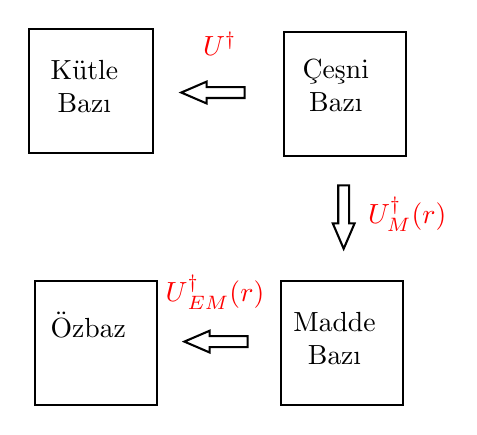
\begin{tikzpicture}[x=0.75pt,y=0.75pt,yscale=-1.5,xscale=1.5]
  %uncomment if require: \path (0,300); %set diagram left start at 0, and has height of 300

  %Shape: Rectangle [id:dp8088308900717263] 
  %\draw   (31,101) -- (70.33,101) -- (70.33,141) -- (31,141) -- cycle ;
  \draw   (30,100) -- (70,100) -- (70,140) -- (30,140) -- cycle ;
  %Right Arrow [id:dp5637298668216818]
  %\draw   (99.33,122.25) -- (87.13,122.25) -- (87.13,124) -- (79,120.5) -- (87.13,117) -- (87.13,118.75) -- (99.33,118.75) -- cycle ;
  \draw   (99.33,122.25) -- (87.13,122.25) -- (87.13,124) -- (79,120.5) -- (87.13,117) -- (87.13,118.75) -- (99.33,118.75) -- cycle ;
  %Shape: Rectangle [id:dp5085257977019034] 
  \draw   (112,101) -- (151.33,101) -- (151.33,141) -- (112,141) -- cycle ;
  %Shape: Rectangle [id:dp33001506333160935] 
  \draw   (111,181) -- (150.33,181) -- (150.33,221) -- (111,221) -- cycle ;
  %Right Arrow [id:dp5718992848093374] 
  \draw   (132.92,150.33) -- (132.92,162.53) -- (134.67,162.53) -- (131.17,170.67) -- (127.67,162.53) -- (129.42,162.53) -- (129.42,150.33) -- cycle ;
  %Right Arrow [id:dp6931270939254744] 
  \draw   (100.33,202.25) -- (88.13,202.25) -- (88.13,204) -- (80,200.5) -- (88.13,197) -- (88.13,198.75) -- (100.33,198.75) -- cycle ;
  %Shape: Rectangle [id:dp069718532513661] 
  \draw   (32,181) -- (71.33,181) -- (71.33,221) -- (32,221) -- cycle ;

    % Text Node
  \draw (138,153) node [anchor=north west][inner sep=0.75pt]  {$\textcolor[rgb]{1,0,0}{U_{M}^{\dagger }( r)}$};                                     
  % Text Node                                                                                                                                                           
  \draw (73,178) node [anchor=north west][inner sep=0.75pt]  {$\textcolor[rgb]{1,0,0}{U}\textcolor[rgb]{1,0,0}{_{EM}^{\dagger }}\textcolor[rgb]{1,0,0}{(}\textcolor[rgb]{1,0,0}{r}\textcolor[rgb]{1,0,0}{)}$};                                                                                                                    
  % Text Node                                                                                                                                                           
  \draw (85,100) node [anchor=north west][inner sep=0.75pt] {$\textcolor[rgb]{1,0,0}{U^{\dagger }}$};                                              
  % Text Node                                                                                                                                                           
  \draw (36,109) node [anchor=north west][inner sep=0.75pt] [align=center] {{Kütle}\\{Bazı}};                                
  % Text Node                                                                                                                                                           
  \draw (117,109) node [anchor=north west][inner sep=0.75pt] [align=center] {{Çeşni}\\{Bazı}};                             
  % Text Node                                                                                                                                                           
  \draw (114,190) node [anchor=north west][inner sep=0.75pt]  [align=center] {{Madde}\\{Bazı}};                             
  % Text Node                                                                                                                                                           
  \draw (36,190) node [anchor=north west][inner sep=0.75pt] [align=center] {{Özbaz}};                              
\end{tikzpicture}
	\caption[Bazlar arası dönüşüm diyagramı.]{Bazlar arası dönüşüm diyagramı.}
	\label{fig:transfDiagram}
\end{figure}

\subsubsection{ANALİTİK ÇÖZÜLEBİLEN ÖZEL DURUMLAR}
\paragraph{}
İkinci ve üçüncü çözüm yöntemlerine geçmeden önce \eqref{eqn:HamiltonyenToplam} numaralı bağıntıda verilen toplam Hamiltonyen'i $ 2\times2 $ matrise indirgememiz gerekmektedir. Bu indirgeme işlemi ile $ \Delta s_{2\theta} $ terimini ihmal ediyoruz. Bu yaklaşıklık, boşluk karışım açısı $ \theta $'nın, küçük değerleri için uygun bir yaklaşımdır. Hamiltonyen'in elektromanyetik etkileşimler dikkate alınarak indirgenmesi iki farklı şekilde olabilir. Birincisi $ e-\bar{x} $ terimlerini alarak, buna $ H_{T,e\bar{x}} $ adı verilecektir, veya $ x-\bar{e} $ terimleri alarak, buna da $ H_{T,x\bar{e}} $ adı verilecektir, indirgeyebiliriz.
\begin{align}
	\label{eqn:Hamiltonyen_T14}H_{T,e\bar{x}} &= \mqty(-\Delta c_{2\theta}+V_{CC}+V_{NC} & \mu B \\ \mu B & \Delta c_{2\theta}-V_{NC}) \\
	\label{eqn:Hamiltonyen_T23}H_{T,x\bar{e}} &= \mqty(\Delta c_{2\theta}+V_{NC} & -\mu B \\ -\mu B & -\Delta c_{2\theta}-V_{CC}-V_{NC})
\end{align}
Hamiltonyen'i $ e-\bar{x} $ ve $ x-\bar{e} $ olarak ayırmamızın sebebi nötrino antinötrino geçişlerinin ancak ve ancak $ e-\bar{x} $ ve $ x-\bar{e} $ arasında olmasıdır. Hamiltonyen'in $ \dyad{\nu_{e}}{\nu_{\bar{e}}} $ ve $ \dyad{\nu_{x}}{\nu_{\bar{x}}} $ bileşenleri sıfırdır. Hangi matrisin ne zaman kullanılması gerektiği ise \ref{sec:sfpRezonansi} numaralı kısımda açıklanacaktır.

Hamiltonyen'i \eqref{eqn:NuKim_EoM_4Mat} numaralı denklemde yerine koyacağız. \eqref{eqn:NuKim_EoM_4Mat} numaralı denklemdeki çeşniler düzeltildikten sonra Hamiltonyenler'in $ ee $ elemanları sıfır olacak şekilde birim matrisle orantılı terimler çıkaracağız.
\begin{align}
	\label{eqn:EoM_14Matris}i\dv{}{r} \mqty(\ket{\nu_{e}} \\ \ket{\nu_{\bar{x}}}) &= 
	\mqty(0 & \mu B \\ \mu B & 2\Delta c_{2\theta}-V_{CC}-2V_{NC}    ) 
	\mqty(\ket{\nu_{e}}\\ \ket{\nu_{\bar{x}}}) \text{ ,}\\
	\label{eqn:EoM_23Matris}i\dv{}{r} \mqty(\ket{\nu_{x}} \\ \ket{\nu_{\bar{e}}}) &= 
	\mqty(0 & -\mu B \\ -\mu B & -2\Delta c_{2\theta}-V_{CC}-2V_{NC} ) 
	\mqty(\ket{\nu_{x}}\\ \ket{\nu_{\bar{e}}}) \text{ .}
\end{align}

Nötrino hareket denklemleri birinci dereceden çiftlenmiş (coupled) diferansiyel denklemlerdir. İki adet birinci dereceden hareket denklemleri, bir adet ikinci dereceden hareket denklemi haline getirilebilir. Basitlik olması açısından $ \nu_{1} \equiv \ket{\nu_{e}} $ ve $ \nu_{2} \equiv \ket{\nu_{x}} $ olarak değiştirilecektir (bu isimlendirme ile kütle tabanını karıştırmayınız.) Bu değişikliklerden sonra $ \nu_{1} $, \eqref{eqn:EoM_14Matris} numaralı denklemin çözümü ve $ \nu_{2} $ ise \eqref{eqn:EoM_23Matris} numaralı denklemin çözümü olacaktır.
\begin{equation}
	\dv[2]{\nu_{i}}{r} + \left(i\kappa_{i}+iP(r) + \frac{\dv{B}{r}}{B(r)}\right) 
    ~\dv{\nu_{i}}{r}+ (\mu B(r))^{2}~ \nu_{i} = 0 \text{ .}
\end{equation}
Burada $ P(r) \equiv -\sqrt{2}G_{F}(1-2Y_{e})N_{b}(r) $ ve $ \kappa_{1,2} \equiv \mp 2\Delta c_{2\theta} $ şeklinde tanımlanmıştır (bu isimlendirme ile olasılık hesabındaki ifadeyi karıştırmayınız.) Bu denklemler çok kullanılan baryon ve manyetik alan profilleri için çözülememektedir. Örneğin, manyetik alanın polinom tipi bir profile, baryon yoğunluğunun eksponansiyel profile sahip olduğu durumda bir çözüm yoktur. En genel çözümü bulmaktansa bu bölümde \emph{sabit manyetik alan} ve \emph{eksponansiyel olarak aynı şekilde azalan baryon ve manyetik alan} profillerini kullanacağız. Hareket denkleminin genel hali aşağıdaki gibi olur.
\begin{equation}\label{eqn:app_diffeqConstB}
    \dv[2]{\nu_{i}}{r} + i\left(\kappa_{i}+P(r)\right) ~\dv{\nu_{i}}{r}+ 
    (\mu B(r))^{2}~ \nu_{i} = 0 \text{ .}
\end{equation}
Bu tip denklemlere \emph{konfluent hipergeometrik} denklemler adı verilir. Denklemlerin bu formu, sadece madde etkileşimi dikkate alındığında da karşımıza çıkar. Sadece madde etkileşimi aldığımız durumda, köşegen olmayan terim $ \mu B $ yerine $ \Delta s_{2\theta} $ ve köşegen terim ise $ \kappa_{i} + P(r) \equiv 2\Delta c_{2\theta} - V_{CC} $ şeklinde gelecektir. Sadece madde etkileşiminde çeşitli baryon (veya elektron) profillerine göre elde edilen çözümler \cite{Ito:1987vy,Toshev:1987jw,Kaneko:1987zza, Notzold:1987cq, Kuo:1989qe,Balantekin:1996ag} numaralı referanslarda verilmiştir. Bu eşdeğerlilik, $ B $'nin uzaklığa bağlı olduğu durumlarda kırılır. 

Sabit dış manyetik alan profili için çözümler \emph{Kummer Fonksiyonları} cinsinden yazılır. Burada,baryon profili $ N_{b}(r) = N_{i}\exp(-\alpha r) $ ve elektron kesri $ Y_{e} $ sabit olacak şekilde madde potansiyeli seçilmiştir. Dikkate alınan bu profillerin ışığında \eqref{eqn:app_diffeqConstB} numaralı denklemlerin çözümleri aşağıdaki gibi olur.
\begin{align}
    \nonumber \nu_{i}(r) & = N_{1}^{\xi^{+}_{i}}~ _{1}F_{1}\left(\xi^{+}_{i}; 
    1+2\xi^{+}_{i}-\kappa_{i};\frac{-iP(r)}{\alpha} \right) \\
    & + N_{2}^{\xi^{-}_{i}} ~ _{1}F_{1}\left(\xi^{-}_{i}; 1+2\xi^{-}_{i}-
    \kappa_{i};\frac{-iP(r)}{\alpha}\right) \text{ ,}
\end{align}
Burada $N_{1,2} \equiv C_{1,2}\frac{i}{\alpha} (\pm \sqrt{2}G_{F}(2Y_{e}-1)n_{i}e^{-\alpha r} )$ ve
\begin{equation}
  \xi^{\mp}_{i} \equiv \frac{i(\kappa_{i} \mp \sqrt{(2\mu B)^{2} + 
  \kappa^{2}_{i} } )}{2\alpha} \text{ ,}
\end{equation}
şeklindedir. Kummer'in fonksiyonları, $ _{1}F_{1}(a;b;z) $, konfluent hipergeometrik denkleminin çözümleridir. $ C_{1,2} $ katsayıları ise çözümlerin limit durumlarından çıkarılır. Örneğin, $ B \rightarrow 0 $ limitinde çeşniler arası salınım olmaması gerekmektedir. Bu ve bunun gibi limitler kullanılarak integral sabitleri belirlenir.

Çözümü olan bir diğer profil ise manyetik alanın ve baryon yoğunluğunun aynı eksponansiyel fonksiyona sahip olduğu durumdur; elektron kesri sabittir. Bu profiller kullanıldığında hareket denklemi aşağıdaki gibi olur.
\begin{equation}\label{eqn:app_exactdiffeqSameAlpha}
    \dv[2]{\nu_{i}}{r} + \left(i\kappa_{i}+iP(r) + \alpha\right)
    \dv{\nu_{i}}{r}+ (\mu B_{i}e^{-\alpha r})^{2}~ \nu_{i} = 0 \text{ .}
\end{equation}
Burada baryon yoğunluğu ve manyetik alan $ \exp(-\alpha r) $ şeklinde uzaklığa bağlıdır. $ B_{i} $ ise başlangıç noktasındaki manyetik alanın büyüklüğüdür. \eqref{eqn:app_exactdiffeqSameAlpha} numaralı denklemin çözümü genelleştirilmiş hipergeometrik fonksiyonlar $ U(a,b,z) $ ve birleşmiş Laguerre polinomları (associated Laguerre polynomials) $ L(n,l,m) $ cinsinden verilir. Açık ifadeleri bu tezin kapsamı dışındadır. Yaklaşık çözümler için \cite{Balantekin:2004tk} numaralı kaynağa ve Demkov-Kunike modeli için \cite{Joshi:2019dcj} numaralı kaynağa bakınız.

\subsubsection{ADYABATİK EVRİM ÇÖZÜMLERİ}
\paragraph{}
Toplam Hamiltonyen \eqref{eqn:HamiltonyenToplam} numaralı denklemin üçüncü ve son çözüm yöntemi ise efektif karışım açısı elde etmektir. Efektif karışım açısının elde edilmesi ile \ref{subsec:MaddeOrtamindaNuEvrimi} numaralı bölümde $ \barparen{\theta}_{M} $ elde edilmesi benzerlik gösterir. Bunun için \eqref{eqn:Hamiltonyen_T14} ve \eqref{eqn:Hamiltonyen_T23} numaralı denklemlerde verilen Hamiltonyenler'i köşegenleştiren dönme (dönüşüm) matrislerini elde etmek gerekecektir. Köşegenleştirme Bloch vektörü yardımıyla yapılacaktır.

$ H_{T,e\bar{x}} $ Hamiltonyen'i için yazılacak olan Bloch vektörü $ \vec{B}_{T,e\bar{x}} $ ve $ H_{T,x\bar{e}} $ için yazılacak olan Bloch vektörü $ \vec{B}_{T,x\bar{e}} $ olarak adlandırılacaktır.
\begin{align}
	\vec{B}_{T,e\bar{x}} =& \mqty(2\mu B & 0 & 2 \Delta c_{2\theta} - V_{CC}-2V_{NC})_{\text{çeşni}} \text{ ,}\\ \vec{B}_{T,x\bar{e}} =& \mqty(2\mu B & 0 & -2 \Delta c_{2\theta} - V_{CC}-2V_{NC})_{\text{çeşni}} \text{.}
\end{align}
Buradan özdeğerler,
\begin{align}
	\label{eqn:Ozdeger_EMetkilesim14}(\lambda_{1,2})_{e\bar{x}} =& \pm M_{EM} + V_{CC}/2 \text{ ,} \\
	\label{eqn:Ozdeger_EMetkilesim23}(\lambda_{1,2})_{x\bar{e}} =& \pm \overline{M}_{EM} - V_{CC}/2
\end{align}
şeklinde yazılır. Burada $ \barparenBig{M}_{EM} = \sqrt{(\mu B)^{2} + (\Delta c_{2\theta} \pm V_{NC} \pm V_{CC}/2)^{2}} $ şeklindedir Özvektörleri veren efektif elektromanyetik karışım açıları ise 
\begin{equation}\label{eqn:theta_EM_hepsi}
	\tan 2\barparen{\theta}_{EM} = \frac{\mu B}{\Delta c_{2\theta} \pm V_{NC} \pm V_{CC}/2} \text{ ,}
\end{equation}
şeklinde yazılır. Madde etkileşiminde elde edilen, $ \theta_{M}(r) $ açısı kullanılarak yazılan $ U_{M}(r) $ dönüşüm matrisi, $ \theta_{EM}(r) $ kullanılarak da da yazılır. Bu yöntem ile elde edilen $ U_{EM}(r) $ matrisi ile \eqref{eqn:U_EM_tedirgenmis} numaralı denklemde verilen $ U_{EM}(r) $ matrisi farklıdır. \eqref{eqn:U_EM_tedirgenmis} numaralı denklemdeki dönüşüm dört çeşni, düşük manyetik alan yaklaşıklığında elde edilmiş, \eqref{eqn:theta_EM_hepsi} numaralı denklemdeki dönüşüm matrisi ise iki çeşni ve düşük $ \Delta s_{2\theta} $ yaklaşıklığında üretilmiştir. Aksi belirtilmedikçe $ \theta_{EM}(r) $ açısından elde edilen dönüşüm matrisi kullanılacaktır.
	
Hamiltonyen'i indirgeyerek elde edilen fiziksel büyüklükler, Hamiltonyen'in $ ex $, $ e\bar{e} $ ve $ x\bar{x} $ terimleri dikkate alınarak da yapılır. Bu işlemleri ayrı ayrı yapmak yerine genelleştirilmiş ifadesini elde etmek mümkündür. \cite{Likhachev:1990ki,Broggini:2012df}. Not edilmelidir ki, birazdan yazılacak olan genelleştirmelerin hepsi alt matrise indirgendikten sonra hesaplanır. Örneğin, $ \alpha=e $ ve $ \beta=\bar{x} $ alındığında \eqref{eqn:EoM_14Matris} numaralı Hamiltonyen ile alakalı büyüklükler elde edilir. $ H_{\alpha\beta} $, \eqref{eqn:HamiltonyenToplam} numaralı Hamiltonyen'in elemanları olmak üzere yaşama olasılığı \cite{Giunti:2014ixa}
\begin{equation}
	P_{\nu_{\alpha} \rightarrow \nu_{\alpha}} = 1 - \sin^{2} 2\theta_{EM} \sin^{2}(\frac{\pi}{L_{EM}}r) \text{ ,}
\end{equation}
şeklinde yazılır. Bu ifade başlangıçta sadece $ \alpha $ çeşnisine sahip nötrinoların yaşama olasılıklarını veren genel ifadedir. Efektif açı $ \theta_{EM} $ yerine $ \theta $ konulduğunda boşlukta ilerleyen $ \alpha $ nötrinolarının yaşama olasılıklarını verir. Bu denklemdeki $ L_{EM} $ salınım dalga boyudur ve aşağıdaki gibi genel olarak tanımlanabilir.
\begin{equation}
	L_{EM}= \frac{2\pi}{\sqrt{4_{H_{\alpha\beta}}^2+(H_{\beta\beta} - H_{\alpha\alpha})^{2}}} \text{ .}
\end{equation}

Hamiltonyen'in elemanlarından salınım dalga boyunu yazabileceğimiz gibi karışım açısı $ \theta_{EM} $ terimini de yazabiliriz. Burada $ \theta_{EM} $ açısının tanjantı değil $ \theta_{EM} $ açısının sinüsünün yazıldığına dikkat edilmelidir \footnote[1]{\cite{Broggini:2012df} numaralı kaynakta efektif açı $ \theta_{EM} $ olarak tanımlanmış ancak \cite{Likhachev:1990ki} numaralı kaynakta $ 2\theta_{EM} $ olarak tanımlanmıştır.}.
\begin{equation}
	\sin 2\theta_{EM} = \frac{H_{\alpha\beta}}{\sqrt{H^{2}_{\alpha\beta} + \qty[(H_{\beta\beta} - H_{\alpha\alpha})/2]^{2}}} \text{ .}
\end{equation}

\eqref{eqn:theta_EM_hepsi} numaralı denklemde verilen efektif karışım açılarını yukarıdaki formülden de elde etmek mümkündür. Hamiltonyen'in $ e\bar{x} $ elemanı için ($ \theta_{EM} $), $ (\alpha,\beta)=(1,4) $ ikilisi ve Hamiltonyen'in $ x\bar{e} $ elemanı için ($ \bar{\theta}_{EM} $), $ (\alpha,\beta)=(2,3) $ ikilisi seçilmelidir.

Efektif elektromanyetik karışım açısının tanjantını \eqref{eqn:theta_EM_hepsi} numaralı denklemde elde etmiştik. \eqref{eqn:V_NC} ve \eqref{eqn:V_CC} numaralı denklemlerdeki madde etkileşim potansiyellerinin ($ V_{CC} $ ve $ V_{NC} $) açık ifadeleri kullanılarak da yazabiliriz. 
\begin{align}
	\tan 2\barparen{\theta}_{EM} = \frac{\mu B}{\Delta c_{2\theta} \pm (\sqrt{2}G_{F}N_{b})(2Y_{e}-1)/2} \text{ .}
\end{align}
Bu açık ifadeleri kullandığımızda, $ Y_{e}=0.5 $'in özel bir değer olduğu görülür. Bu özel değerde, efektif karışım açısı aşağıdaki gibi verilir.
\begin{equation}
	\eval{\tan 2\barparen{\theta}_{EM}}_{Y_{e}=0.5} = \frac{\mu B}{\Delta c_{2\theta}} \text{.}
\end{equation}

$ Y_{e}=0.5 $ değeri için efektif elektromanyetik karışım açısı içerisinde madde etkileşim terimi bulunmamaktadır. Bu limitte Hamiltonyen'i $ 2\times2 $ boyutlu matrise indirgerken dikkatli olunması gerekmektedir. $ Y_{e}=0.5 $ limitinde \eqref{eqn:EoM_14Matris} ve \eqref{eqn:EoM_23Matris} numaralı Hamiltonyenler'i tekrar yazalım.
\begin{align}
	\label{eqn:EoM_14MatrisYe05}\eval{H_{T,e\bar{x}}}_{Y_e=0.5} &= 
	\mqty(0 & \mu B \\ \mu B & 2\Delta c_{2\theta}) \text{ ,}\\
	\label{eqn:EoM_23MatrisYe05}\eval{H_{T,x\bar{e}}}_{Y_e=0.5}&= 
	\mqty(0 & -\mu B \\ -\mu B & -2\Delta c_{2\theta}) \text{ .}
\end{align}
Yukarıdaki yazılan iki matris de aynıdır. Hamiltonyen'i indirgerken boşluk salınımlarının etkisinin çok düşük olacağı varsayılmıştı. $ Y_{e}=0.5 $ limitinde bu varsayım, sadece ve sadece $ \mu B \gg 2\Delta c_{2\theta}$ yaklaşıklığında geçerli olacaktır. %Madde etkileri gittiğinde $ \Delta s_{2\theta} $ terimini sadece $ \mu B $ ile kıyaslayarak ihmal edebiliriz.

Son olarak bu limitte özdeğerler de yazılabilir. Özdeğerler her iki Hamiltonyen için aynı olacaktır.
\begin{equation}\label{eqn:eigValTotal_Ye05}
	\eval{(\lambda_{1,2})}_{Y_{e}=0.5} = \pm\sqrt{(\mu B)^{2} + (\Delta c_{2 \theta})^{2}}\text{ .}
\end{equation}
Dikkatli bakıldığında $ \theta = 0 $ için \eqref{eqn:eigValTotal_Ye05} ve \eqref{eqn:eigValNuEm} numaralı denklemler aynıdır. 

Sonuç olarak nötrino elektromanyetik alan etkileşimini ve nötrino madde etkileşimini dikkatte aldığımızda, $ Y_{e}=0.5 $ için madde etkileri neredeyse yok olmaktadır. Bu limit astrofiziksel ortamlar için önemlidir, çünkü $ Y_{e}=0.5 $, nötr bir ortam için proton ve nötron sayılarının eşitliği anlamına gelir.

Bir sonraki bölümde nötrino-nötrino etkileşimlerinden kaynaklanan terimler incelenecektir. Astrofiziksel ortamlarda yani nötrino yoğunluğunun çok yüksek olduğu yerlerde nötrino-nötrino etkileşimlerinden bahsetmek mümkün olacaktır.

\section{NÖTRİNO ÖZ-KIRILIMI}\label{sec:notrinoOzKirilimi} % Self-Refraction

Nötrinoların Standart Model etkileşim tesir kesitleri diğer temel parçacıklara nazaran çok küçüktür \cite{Formaggio:2012cpf}. Buna rağmen ÇÇSN, nötron yıldızı birleşmeleri veya kozmoloji gibi nötrino akısının (flux) çok yüksek olduğu fenomenlerde nötrino - nötrino etkileşimleri söz konusu olabilir \cite{Berryman:2022hds}. Nötrino - nötrino etkileşmelerinin efektif Hamiltonyen'i diğer etkileşimler gibi değildir ve ortamın geometrisine bağlıdır. Bu bölümde nötrino - nötrino etkileşimlerini inceleyeceğiz. Literatürde nötrino - nötrino etkileşimleri ismi yerine nötrino öz-etkileşimi \cite{Berryman:2022hds} (self-interaction), nötrino öz-kırılımı (self-refraction) \cite{Pehlivan:2010zz,Friedland:2010sc}, nötrino kolektif çeşni değişimi \cite{Chakraborty:2016yeg} gibi isimler kullanılmaktadır. Tezin geri kalanında nötrino - nötrino etkileşimleri yerine nötrino öz-kırılımı ifadesi kullanılacaktır.

Nötrino madde etkileşimlerinden ve nötrino elektromanyetik etkileşimlerden farklı olarak nötrino öz-kırılımı dinamik bir etkileşimdir. Nötrinolar arka plandaki madde veya manyetik alanla etkileşirken, etkileşilen madde ve manyetik alanın değişmediği varsayılmıştır. Bu durum etkileşimleri statik yapar. Nötrino öz-kırılımında ise test nötrinosu, diğer nötrinoların oluşturduğu nötrino alanı ile etkileşir. Bu etkileşimin hemen ardından nötrinoların tüm çeşni yapısı değişecektir. Bunun sonucunda arka plandaki nötrino profili her adımda değişecektir. Bu nedenden ötürü nötrino öz-kırılma Hamiltonyen'i içerisinde nötrino alanının integrali bulunmaktadır. Aynı zamanda bu dinamik değişim hareket denklemlerini de birbirine bağlar. Çeşni evrimini veren \eqref{eqn:NuKim_LiouvilleVonNeumann} numaralı denklem seti birbirine bağlı yani çiftlenmiş (coupled) olacaktır. Buna ek olarak, nötrino profilinin dinamik olması, \eqref{eqn:NuKim_LiouvilleVonNeumann} numaralı denklem setini doğrusal olmayan (non linear) diferansiyel denklem haline getirecektir.

Nötrino öz-kırılım Hamiltonyen'i aşağıdaki gibi yazılır \cite{Sigl:1993ctk}.
\begin{align}\label{eqn:Hamil_nunuOperator}
	\nonumber \hat{H}_{\nu\nu}(r)= & \sum_{\alpha\beta=e,x,\bar{e},\bar{x}} (H_{\nu\nu})_{\alpha\beta} \dyad{\nu_{\alpha}}{\nu_{\beta}} \text{ ,}\\ 
	=&\sqrt{2} G_{F} D(r)\sum_{\alpha,\beta = e,x} \qty[\int \qty[\rho_{\alpha\beta}(E,r)-\rho_{\bar{\alpha}\bar{\beta}}(E,r)]\dd{E}] \qty(\dyad{\nu_{\alpha}}{\nu_{\beta}}-\dyad{\nu_{\bar{\alpha}}}{\nu_{\bar{\beta}}}) \text{ .}
\end{align}
Burada $ D(r) $, sistemin geometrisinden gelen katkıdır ve \ref{subsec:geometri} numaralı bölümde tartışılacaktır. Öz-kırılım Hamiltonyen operatörü Standart Model çiflenim sabitine göre yazılmıştır. Bu operatör çeşni tabanında yazılmıştır, ancak öz-kırılım Hamiltonyen'i tabandan bağımsızdır. Yani üniter dönüşümler altında değişmez (invariant) kalır. Matris temsili $ (H_{\nu\nu})_{\alpha\beta} $ ise

{\small
\begin{equation}
	(H_{\nu\nu})_{\alpha\beta}(r) = \sqrt{2} G_{F} D(r) \int \dd{E} \mqty((\rho_{ee}-\rho_{\bar{e}\bar{e}}) & (\rho_{ex}-\rho_{\bar{e}\bar{x}}) & 0 & 0\\ (\rho_{xe}-\rho_{\bar{x}\bar{e}}) & (\rho_{xx}-\rho_{\bar{x}\bar{x}}) & 0 & 0\\ 0 & 0 & (\rho_{\bar{e}\bar{e}} -\rho_{ee}) & (\rho_{\bar{e}\bar{x}} -\rho_{ex}) \\ 0 & 0 & (\rho_{\bar{x}\bar{e}} -\rho_{xe}) & (\rho_{\bar{x}\bar{x}} -\rho_{xx})) \text{ ,}
\end{equation}}
şeklinde yazılır. Hamiltonyen matrisine bakıldığında nötrino - antinötrino geçişleri bulunmamaktadır. Öz-kırılım Hamiltonyen'i sadece ileri saçılmaları (forward scattering) dikkate almıştır. İleri saçılmalar, öz-kırılım Hamiltonyen'ine en büyük katkıyı getirecektir \cite{Cherry:2013mv, Volpe:2015rla}

Nötrino öz-kırılımının çeşni evrimine etkisi ele alınan sistemin geometrisine göre çeşitlilik gösterir. Örneğin, küresel bir kaynaktan çıkan nötrinolar için etkileşim geometrisi küresel simetrik olur. Ortamda var olan nötrinolar belli bir açıyla öz-kırılım potansiyelinin içerisine girer ve birbirleri ile etkileşirler. Bu geometriye örnek olarak ÇÇSN gösterilebilir. Bir diğer taraftan iki nötron yıldızının birleşmesi gibi iki kaynaktan çıkan nötrinoların oluşturduğu geometri daha karmaşıktır. Bu tezde nötrinoların ÇÇSN'nın merkezinde oluşan proto-nötron yıldızından çıktığı varsayılacaktır. Öz-kırılım geometrisi ise \ref{subsec:geometri} numaralı bölümde ayrıntılı olarak ele alınmıştı.

Nötrino öz-kırılımı için efektif karışım açısı veya Bloch vektörü yazmak olanaksızdır, çünkü çözülecek olan hareket denklemi yoğunluk matrisinin kendisine bağlıdır. Bu nedenle, öz-kırılım Hamiltonyen'i dikkate alındığında hareket denklemlerinin analitik çözümü bulunmamaktadır. Buna rağmen iki çeşni için çeşitli simetriler ve değişmezler (invariants), yani korunan büyüklükler hesaplanabilir \cite{Pehlivan:2011hp}. Simetriler ve korunan büyüklükler bu tezde bahsedilmeyecek olan polarizasyon vektörü ve özellikleri kullanılarak hesaplanır \cite{fackler1986Massive}. Analitik çözümün eğilimini belirlemek adına hareket denklemini doğrusallaştırılıp (linearization) incelemek de literatürde kullanılan bir yöntemdir. Bu doğrusallaştırma neticesinde çeşitli analizler yapılabilir \cite{Chakraborty:2014lsa, Chakraborty:2019wxe, Xiong:2021dex}. Çeşitli sayısal çözümler ve spektral ayrışma/ spektral yer değiştirme (spectral split/spectral swap) gibi kolektif etkiler \ref{ch:simulasyonlar} numaralı bölümde ayrıntılı olarak ele alınacaktır.